\documentclass[oneside]{book}

\usepackage{amsmath, amsthm, amssymb, amsfonts}
\usepackage{thmtools}
\usepackage[english]{babel}
\usepackage{cancel}
\usepackage{enumerate}
\usepackage{enumitem}
\usepackage{environ}
\usepackage{epigraph}
\usepackage{etoolbox}
\usepackage{float}
\usepackage{framed}
\usepackage{geometry}
\usepackage{graphics}
\usepackage{graphicx}
\graphicspath{ {./img/} }
\usepackage{hhline}
\usepackage{hyperref}
\usepackage[utf8]{inputenc}
\usepackage{listings}
\usepackage{mathrsfs}
\usepackage{setspace}
\usepackage{slashed}
\usepackage[dvipsnames]{xcolor}
\usepackage{tikz-cd}
\usepackage{tcolorbox}
\tcbuselibrary{theorems,skins,breakable}

\setstretch{1.2}
\geometry{
    textheight=9in,
    textwidth=5.5in,
    top=1in,
    headheight=12pt,
    headsep=25pt,
    footskip=30pt
}

\newcommand{\harp}{\overset{\rightharpoonup}}
\newcommand{\hook}{\overset{\hookrightarrow}}
\newcommand{\preim}{\text{preim}}
\newcommand{\dif}{\text{d}}
\newcommand{\id}{\text{id}}
\newcommand{\tr}{\text{tr}}
\newcommand{\addrow}[1]{#1\\}
\newcommand{\vect}[1]{
\begin{bmatrix}
\forcsvlist\addrow{#1}
\end{bmatrix}}

% Variables
\def\notetitle{Analysis of the Three-body Problem
}
\def\notesubtitle{Geometry, Chaos and Simulation}
\def\noteauthor{
    Avery Cormier, Siddhartha Bhattacharjee, ZiLing Chen \\
    AMATH 271 Final Project \\
    Instructor: Francis Poulin \\
    University of Waterloo
    }
\def\notedate{Fall 2023}

% The theorem system and user-defined commands
% Theorem System
% The following boxes are provided:
%   Definition:     \defn 
%   Theorem:        \thm 
%   Lemma:          \lem
%   Corollary:      \cor
%   Proposition:    \prop   
%   Claim:          \clm
%   Fact:           \fact
%   Proof:          \pf
%   Example:        \ex
%   Remark:         \rmk (sentence), \rmkb (block)
% Suffix
%   r:              Allow Theorem/Definition to be referenced, e.g. thmr
%   p:              Add a short proof block for Lemma, Corollary, Proposition or Claim, e.g. lemp
%                   For theorems, use \pf for proof blocks

% Definition
\newtcbtheorem[number within=section]{mydefinition}{Definition}
{
    enhanced,
    frame hidden,
    titlerule=0mm,
    toptitle=1mm,
    bottomtitle=1mm,
    fonttitle=\bfseries\large,
    coltitle=black,
    colbacktitle=green!20!white,
    colback=green!10!white,
}{defn}

\NewDocumentCommand{\defn}{m+m}{
    \begin{mydefinition}{#1}{}
        #2
    \end{mydefinition}
}

\NewDocumentCommand{\defnr}{mm+m}{
    \begin{mydefinition}{#1}{#2}
        #3
    \end{mydefinition}
}

% Theorem
\newtcbtheorem[use counter from=mydefinition]{mytheorem}{Theorem}
{
    enhanced,
    frame hidden,
    titlerule=0mm,
    toptitle=1mm,
    bottomtitle=1mm,
    fonttitle=\bfseries\large,
    coltitle=black,
    colbacktitle=cyan!20!white,
    colback=cyan!10!white,
}{thm}

\NewDocumentCommand{\thm}{m+m}{
    \begin{mytheorem}{#1}{}
        #2
    \end{mytheorem}
}

\NewDocumentCommand{\thmr}{mm+m}{
    \begin{mytheorem}{#1}{#2}
        #3
    \end{mytheorem}
}

% Lemma
\newtcbtheorem[use counter from=mydefinition]{mylemma}{Lemma}
{
    enhanced,
    frame hidden,
    titlerule=0mm,
    toptitle=1mm,
    bottomtitle=1mm,
    fonttitle=\bfseries\large,
    coltitle=black,
    colbacktitle=violet!20!white,
    colback=violet!10!white,
}{lem}

\NewDocumentCommand{\lem}{m+m}{
    \begin{mylemma}{#1}{}
        #2
    \end{mylemma}
}

\newenvironment{lempf}{
	{\noindent{\it \textbf{Proof for Lemma}}}
	\tcolorbox[blanker,breakable,left=5mm,parbox=false,
    before upper={\parindent15pt},
    after skip=10pt,
	borderline west={1mm}{0pt}{violet!20!white}]
}{
    \textcolor{violet!20!white}{\hbox{}\nobreak\hfill$\blacksquare$} 
    \endtcolorbox
}

\NewDocumentCommand{\lemp}{m+m+m}{
    \begin{mylemma}{#1}{}
        #2
    \end{mylemma}

    \begin{lempf}
        #3
    \end{lempf}
}

% Corollary
\newtcbtheorem[use counter from=mydefinition]{mycorollary}{Corollary}
{
    enhanced,
    frame hidden,
    titlerule=0mm,
    toptitle=1mm,
    bottomtitle=1mm,
    fonttitle=\bfseries\large,
    coltitle=black,
    colbacktitle=orange!20!white,
    colback=orange!10!white,
}{cor}

\NewDocumentCommand{\cor}{+m}{
    \begin{mycorollary}{}{}
        #1
    \end{mycorollary}
}

\newenvironment{corpf}{
	{\noindent{\it \textbf{Proof for Corollary.}}}
	\tcolorbox[blanker,breakable,left=5mm,parbox=false,
    before upper={\parindent15pt},
    after skip=10pt,
	borderline west={1mm}{0pt}{orange!20!white}]
}{
    \textcolor{orange!20!white}{\hbox{}\nobreak\hfill$\blacksquare$} 
    \endtcolorbox
}

\NewDocumentCommand{\corp}{m+m+m}{
    \begin{mycorollary}{}{}
        #1
    \end{mycorollary}

    \begin{corpf}
        #2
    \end{corpf}
}

% Proposition
\newtcbtheorem[use counter from=mydefinition]{myproposition}{Proposition}
{
    enhanced,
    frame hidden,
    titlerule=0mm,
    toptitle=1mm,
    bottomtitle=1mm,
    fonttitle=\bfseries\large,
    coltitle=black,
    colbacktitle=yellow!30!white,
    colback=yellow!20!white,
}{prop}

\NewDocumentCommand{\prop}{+m}{
    \begin{myproposition}{}{}
        #1
    \end{myproposition}
}

\newenvironment{proppf}{
	{\noindent{\it \textbf{Proof for Proposition.}}}
	\tcolorbox[blanker,breakable,left=5mm,parbox=false,
    before upper={\parindent15pt},
    after skip=10pt,
	borderline west={1mm}{0pt}{yellow!30!white}]
}{
    \textcolor{yellow!30!white}{\hbox{}\nobreak\hfill$\blacksquare$} 
    \endtcolorbox
}

\NewDocumentCommand{\propp}{+m+m}{
    \begin{myproposition}{}{}
        #1
    \end{myproposition}

    \begin{proppf}
        #2
    \end{proppf}
}

% Claim
\newtcbtheorem[use counter from=mydefinition]{myclaim}{Claim}
{
    enhanced,
    frame hidden,
    titlerule=0mm,
    toptitle=1mm,
    bottomtitle=1mm,
    fonttitle=\bfseries\large,
    coltitle=black,
    colbacktitle=pink!30!white,
    colback=pink!20!white,
}{clm}


\NewDocumentCommand{\clm}{m+m}{
    \begin{myclaim*}{#1}{}
        #2
    \end{myclaim*}
}

\newenvironment{clmpf}{
	{\noindent{\it \textbf{Proof for Claim.}}}
	\tcolorbox[blanker,breakable,left=5mm,parbox=false,
    before upper={\parindent15pt},
    after skip=10pt,
	borderline west={1mm}{0pt}{pink!30!white}]
}{
    \textcolor{pink!30!white}{\hbox{}\nobreak\hfill$\blacksquare$} 
    \endtcolorbox
}

\NewDocumentCommand{\clmp}{m+m+m}{
    \begin{myclaim*}{#1}{}
        #2
    \end{myclaim*}

    \begin{clmpf}
        #3
    \end{clmpf}
}

% Fact
\newtcbtheorem[use counter from=mydefinition]{myfact}{Fact}
{
    enhanced,
    frame hidden,
    titlerule=0mm,
    toptitle=1mm,
    bottomtitle=1mm,
    fonttitle=\bfseries\large,
    coltitle=black,
    colbacktitle=purple!20!white,
    colback=purple!10!white,
}{fact}

\NewDocumentCommand{\fact}{+m}{
    \begin{myfact}{}{}
        #1
    \end{myfact}
}


% Proof
\NewDocumentCommand{\pf}{+m}{
    \begin{proof}
        [\noindent\textbf{Proof.}]
        #1
    \end{proof}
}

% Example
\newenvironment{example}{%
    \par
    \vspace{5pt}
	\begin{minipage}{\textwidth}
		\noindent\textbf{Example.}
		\tcolorbox[blanker,breakable,left=5mm,parbox=false,
	    before upper={\parindent15pt},
	    after skip=10pt,
		borderline west={1mm}{0pt}{cyan!10!white}]
}{%
		\endtcolorbox
	\end{minipage}
    \vspace{5pt}
}

\NewDocumentCommand{\ex}{+m}{
    \begin{example}
        #1
    \end{example}
}


% Remark
\NewDocumentCommand{\rmk}{+m}{
    {\it \color{blue!50!white}#1}
}

\newenvironment{remark}{
    \par
    \vspace{5pt}
    \begin{minipage}{\textwidth}
        {\par\noindent{\textbf{Remark.}}}
        \tcolorbox[blanker,breakable,left=5mm,
        before skip=10pt,after skip=10pt,
        borderline west={1mm}{0pt}{cyan!10!white}]
}{
        \endtcolorbox
    \end{minipage}
    \vspace{5pt}
}

\NewDocumentCommand{\rmkb}{+m}{
    \begin{remark}
        #1
    \end{remark}
}


\newcommand{\lcm}{\operatorname{lcm}}



% ------------------------------------------------------------------------------

\begin{document}
\title{\textbf{
    \LARGE{\notetitle}} \\
    \Large{\notesubtitle} \vspace* {10\baselineskip}}
\author{\noteauthor}
\date{\notedate}

\maketitle
\newpage

\chapter*{Abstract}
In this project, we examine the physical evolution and stability of three-body systems. 

We introduce the $N$-body problem and capture a bird's eye view of the geometry underlying systems in the form of physical space, configuration space, state space and the relationships between them elucidated using algebraic topological notions such as loop spaces and homotopy theory.

After laying out the theoretical backdrop, we steer our exposition to investigate various aspects of the three-body problem, starting with the local evolution of error at given states. We also simulate, in python, the evolution of the entire system. Finally, we analyze a periodic solutions. Overall, we accomplish this by studying the three-body problem mathematically. The system will be evolving over time with given variables of mass, position, and velocity, for each body in three
dimensions. 

First, we find the 9 differential equations using Newtonian mechanics. We then convert this to a 1st order DE. This will allow us to use computational methods to simulate the three-body system given initial values. By finding a next approximate state we can correct the accuracy by accounting for conserved quantities. We do this by adjusting our generalized coordinates in the direction to most quickly change conserved quantities. This direction is
found by the gradient of our conserved quantities. This addition to the computational method ensures that energy, momentum, angular momentum are conserved when constraining to the center of mass to be the origin. 

Once we have the DE we can linearize it and write a program to find the eigenvectors and eigenvalues. This
will allow use to solve for error locally. If the eigenvalues are negative, then that component of the error goes to 0. If the eigenvalue is positive, then that component of the error grows exponentially. This will
tell where there are regions of chaos and stability. By accumulating this value of stability across the path
we can get a cumulative estimate of the stability of the system over those states.

\tableofcontents
\newpage

% ------------------------------------------------------------------------------

\chapter{Introduction}

\epigraph{The present is big with the future, the future might be read in the past, the distant is expressed in the near.}{\textit{Gottfried Leibniz}}

\section{Setting}

A large class of problems that physics solves is the $N$-body problem: that of predicting the \hyperref[configuration_space]{configurations} of $N$ bodies at some point of time, given the configurations at some other time as well as the interactions and dynamics of the bodies (encoded in the action, Lagrangian, Hamiltonian, Hamilton's principle function or one of such equivalent quantities).

Classical mechanics is a chassis for dealing with and solving such kinds of problems, without incorporating the vagaries of quantum mechanics. One of the frameworks that can be built around this skeleton of classical mechanics is non-holonomic mechanics, which is described in \hyperref[appendix_A]{Appendix A}. This framework is further fleshed out with the calculus of variations to talk about how configurations actually evolve with time, giving rise to the Lagrangian, Hamiltonian, Poisson bracket, Hamilton-Jacobi, Maupertius-Jacobi and other equivalent formulations of non-holonomic classical mechanics.

Most of this introduction builds arounds the concepts constructed in the appendix mentioned, in order to move on to analysis and computations for the 3-body problem.

\newpage
\section{Collisions and Non-holonomy}
\label{avoiding_collisions}

Consider a system of $N$ bodies occupying, at each instant of time $t \in \mathbb{R}$, a rigid region of space\footnote{Given a set $A$, $\mathcal{P}(A)$ denotes its \textbf{power set} i.e. the set of all subsets of $A$, \\
$$U \in \mathcal{P}(A) \Longleftrightarrow U \subseteq A$$} $V_{\alpha} : \mathbb{R} \to \mathcal{P}(\mathbb{R}^{D})$ with $\alpha = 1, 2, \dots, N$. Assuming that none of these bodies are made of simpler bodies for the purposes of tracking their motion, these regions are \hyperref[path_connectedness_defn]{path connected} which intuitively means that it does not contain disjoint regions and that any two points in it are accessible to each other via some path that need not leave the body. Rigidity would entail the time-invariance of the distances between every pair of points in the body. Formally, this can be modelled as a \hyperref[holonomic_constraint_defn]{holonomic constraint} as follows. 

We imagine each region of space $V_{\alpha}(t)$ occupied by a body as a collection of mutually disjoint regions $U_{i}(t)$ labelled by lower case Latin indices as $i = 1, 2, \dots, \nu(\alpha)$,

\begin{align*}
i \neq j \implies U_i(t) \cap U_j(t) & = 0 \\
V_{\alpha}(t) & = \underset{i=1}{\overset{\nu(\alpha)}{\bigcup}} U_i(t)
\end{align*}

In other words, $\{ U_i(t) \}$ is a \textbf{partition} for $V_{\alpha}(t)$. Each part $U_i(t)$ can also be viewed as an equivalence class,

\begin{align*}
\forall \: x, y \in \mathbb{R}^D : x \sim y & \Longleftrightarrow x, y \in U_i(t) \\
U_i(t) = [\pmb{\rho}_i(t)] & \text{ such that } \forall \: t \in \mathbb{R} : \pmb{\rho}_i(t) \in U_i(t)
\end{align*}

Thus, we can \emph{represent} each part of the region a body occupies by a \hyperref[positions_defn]{position} $\rho_i : \mathbb{R} \to \mathbb{R}^D$.

The region $V_{\alpha}(t)$ is \textbf{rigid} when the distances between the points representing its parts do not change,

$$f(\rho_1(t), \rho_2(t), \dots, \rho_{\nu(\alpha)}(t)) = 0$$

where,

$$f(\rho_1(t), \rho_2(t), \dots, \rho_{\nu(\alpha)}(t)) = \sum_{i=1}^{\nu(\alpha)} \sum_{j=1}^{\nu(\alpha)} \| \pmb{\rho}_i(t) - \pmb{\rho}_j(t) \|^2$$

When the above function is zero, so is the sum of the squares of distances between all pairs of regions, therefore, each distance must be zero. Even though the above constraint looks \hyperref[semi_holonomic_constraint_defn]{semi-holonomic}, since it dictates rigidity, one can always pick a reference frame where the region occupied by the $\alpha^{\text{th}}$ body is stationary, making the contraint holonomic. However, a problem is that there is generally no frame where this static nature of a body is true for \emph{all} the bodies occupying $\{ V_\alpha(t) \}$. Therefore, the constraint where all of these regions are simultaneously rigid is semi-holonomic; and semi-holonomic constraints generally make systems \hyperref[non_holonomy_defn]{non-holonomic}.

There is an additional layer of complexity that comes with rigidity, as follows. When we track each body (which is, really, a time-dependent path connected region as discussed) using only the position of a representative location always within the body, no two separate bodies may approach each other so close that they share some common region. This undesirable situation, which would contradict rigidity, is a \textbf{collision} at some time $t$,

$$\exists \: t \in \mathbb{R}, \alpha, \beta : V_{\alpha}(t) \cap V_{\beta}(t) \neq \emptyset$$

Therefore, complete rigidity is not only expressed by a collection of semi-holonomic constraints for each body, but an additional statement about the entire system of bodies wherein no two bodies can collide. This is a complicated setup, and one that makes non-holonomy inevitable as an artefact of tracking entire bodies with positions of single points in them. 

We will not prove the above relationship between non-holonomy and collisions as the purpose of this section is to justify choosing a \emph{holonomic} setup and how the point particle $N$-body subclass of $N$-body problems achieves it meaningfully. However, the intuition for non-holonomy emerging from collisions is simply that a non-point body contains more \hyperref[states_defn]{states} than configurations. Here, the states are the positions of all subregions $U_i(t)$ in the body, which cannot be sufficiently captured in a single representative position as interactions with other bodies could entail collisions, which happen at the surface level of rigid bodies, with the surfaces involving complicated attributes such as size, shape and orientation. The configuration, on the other hand, is the much simpler position of a representative point always contained in the body. By definition, more states than configurations leads to non-holonomy.

A good reason for entirely curtailing non-holonomy from analyzing a specific $N$-body problem, at least initially, is to not have to deal with the complexities introduced by rigidity as discussed above. Such details would make it initially difficult to glean the essential features of $N$-body problems shared by holonomic and non-holonomic systems alike. For example, collisions between finitely-sized bodies tracked using just points in them would appear unsmooth as the bodies can continuously approach each other but would abruptly not be able to (and reflect off, to preserve total linear momentum). Therefore, the calculus of trajectories of such nature would entail rigorous care which makes analyzing solutions an extensive enterprise.

The question then remains of how to 'holonomize' the $N$-body problem in a way that keeps as many of its features, as possible, intact.

\newpage
\section{Particles and Holonomization}

A simple enough answer to the above question is to consider situations when bodies represented by single points is a good approximation. This can happen in general when the bodies travel distances much larger than their size. In such a scenario, microscopic details about each body's surface would not be important for collision considerations.

The idea being described here is simply that of a formal particle or simply a \textbf{particle}: a body whose trajectories are much bigger than its own size. 

\rmkb{Note that point particles are a \emph{subclass} of the formal particles described above. In a sense described below, particles are approximately point particles as far as $N$ body dynamics are concerned.}

Without getting into the gory mathematics establishing the connection between this notion of size comparison of trajectories and bodies, and holonomy, a relatively simple partial argument is as follows. By their very nature, formal particles would not undergo 'very' unsmooth collisions; two particles can get close to each other and abruptly bounce off but since their sizes are much smaller than trajectories, this collision is approximately equivalent to a setup where they were just the points representing them, wherein the collision would simply place the points next to each other and not 'inside' each other as this very notion of 'inside' has been removed. In other words, particles make notions of surface structure irrelavant for the dynamics of $N$ bodies, thereby reducing the state space to the same 'size' as the configuration space of points representing the bodies. And so, this procedure of 'holonomization' says, "\textit{let there be holonomy!}".

\newpage
\section{Orbits}

The previous part of the introduction, in conjunction with \hyperref[appendix_A]{appendix A}, is a theoretical background for the analysis and computation to come for specifically looking at the 3-body problem from a pragmatic point of view. In order to complete this section and move on to to the pragmatic section, we lay out the idea of how orbits exist as solutions of $N$-body problems. The backdrop for this is that of \hyperref[loop_spaces]{loop spaces} described in the mentioned appendix.

Lagrangian and other formulations of analytical mechanics begin with the principle of stationary action which says that on-shell or 'natural' trajectories $q \in \mathcal{Q}^{\mathbb{R}}$ (where $\mathcal{Q}$ is the \hyperref[configuration_space]{configuration space}) are those about which first-order perturbations keep the action (which is a linear functional $\mathcal{Q}^{\mathbb{R}} \to \mathbb{R}$) stationary up to first-order i.e. $\delta S[q] = 0$.

Now, as $S$ is a linear functional, \hyperref[concatenation]{concatenations} of trajectories $\gamma_1, \gamma_2$ which are path component equivalent satisfy,

$$S[\tilde{\gamma}_2 * \gamma_1] = S[\gamma_1] - S[\gamma_2]$$

But if $\gamma_1, \tilde{\gamma}_2$ both keep the action stationary, so must their difference and hence their concatenation,

\begin{align*}
\delta S[\gamma_1] & = \delta S[\gamma_2] = 0 \\
\delta S[\gamma_1] - \delta S[\gamma_2] & = \delta S[\tilde{\gamma}_2 * \gamma_1] = 0
\end{align*}

Therefore, the existence of \hyperref[homotopy_equivalence_curves]{homotopic} solutions guaruntees that of orbits, since $\tilde{\gamma}_2 * \gamma_1$ is a \hyperref[loop_defn]{loop}. Now, if we assume $\mathcal{Q}$ has no \hyperref[hole_defn]{holes}, it is \hyperref[contractibility_defn]{contractible} and hence, \hyperref[simple_connectedness_defn]{simply connected} which allows homotopic curves to always exist between points, leading to loops.

Now that we have informally\footnote{formalizing this would involve proving that on-shell homotopic curves exist.} seen how orbits can come up in $N$-body problems, we can justify analyzing them and their stability, which qualifies whether perturbations of orbits deviate from orbits (instability) or stay 'close' to the orbits (Lyapunov stability)\footnote{A weaker notion of stability is asymptotic stability where perturbations of orbits eventually converge to the orbits.}.

\chapter{Equations}

\section{Equations of motion}
To begin with a solution to the problem we need to get the equations of motion\\
\begin{figure}[h]
\centering
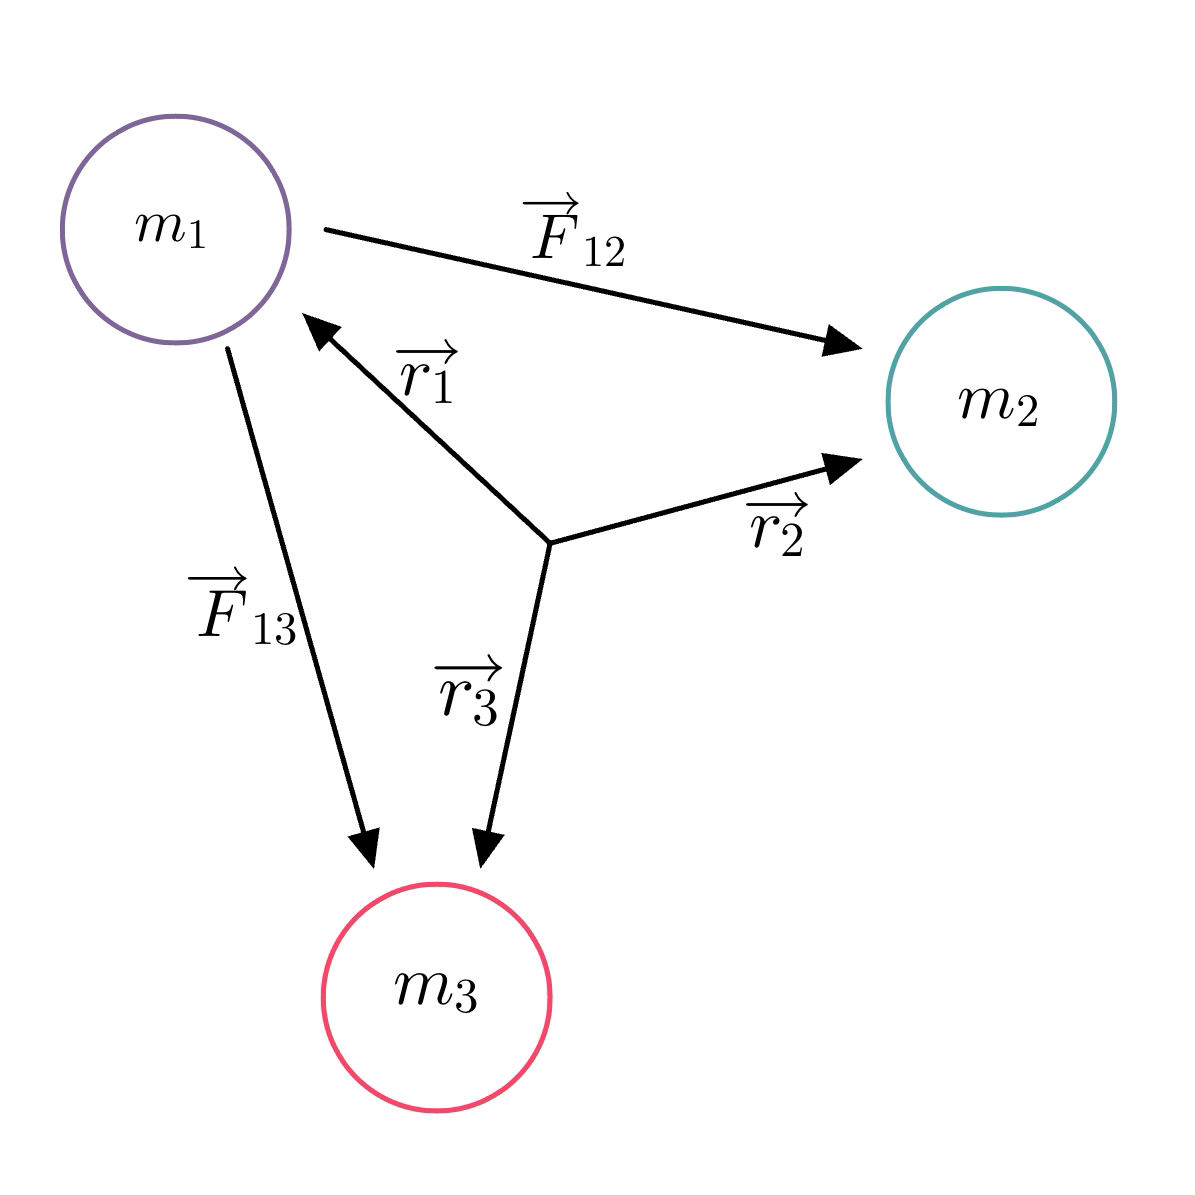
\includegraphics[scale = 0.15]{3_Body_diagram}
\label{fig:1}\caption{The three bodies (ZiLing, Sid, \& Avery)}
\end{figure}

Consider the three bodies set up as shown in figure 1 \ref{fig:1}, and recall Newton's force equation \[\vec{F} = \dfrac{GMm}{r^2}\hat{r}\]
Applying this to object one tells us that \begin{align}
\vec{F}^{net}_1 = \vec{F}_{12} + \vec{F}_{13} = gm_1\left(\dfrac{m_2}{\|\vec{r}_2 - \vec{r}_1\|^3}(\vec{r}_2 - \vec{r}_1) + \dfrac{m_3}{\|\vec{r}_3 - \vec{r}_1\|^3}(\vec{r}_3 - \vec{r}_1)\right) \label{Force Equation}
\end{align}
Using Newton's $\vec{F} = m\vec{a} = m\frac{\partial^2}{\partial t^2}\vec{r}$ we get
\[\frac{\partial^2}{\partial t^2}\vec{r}_i = g\sum_{j\ne i}\left(\dfrac{m_j}{\|\vec{r}_j - \vec{r}_i\|^3}(\vec{r}_j - \vec{r}_i)\right)\]
Notice that by introducing $\vec{v} = \frac{\partial}{\partial t}\vec{r}$ we get a system of first order equations:
\begin{align}
\vec{v}_i = \frac{\partial}{\partial t}\vec{r}_i,\ \frac{\partial}{\partial t}\vec{v}_i = g\sum_{j\ne i}\left(\dfrac{m_j}{\|\vec{r}_j - \vec{r}_i\|^3}(\vec{r}_j - \vec{r}_i)\right) \label{Main differential equation}
\end{align}

\section{Conserved quantities}
To perform computation and analysis it is useful to have reference to conserved quantities. In the following we find conserved Energy, linear momentum, angular momentum. (And also Center of mass since we can assume that momentum is 0)\\

Notice that we can get Potential Energy by integrating both sides of our force equation\ref{Force Equation}. This gives us
\[U = \sum_{i}\int\vec{F}_i\cdot\vec{dx} = \frac{1}{2}\sum_{i,j:\ j\ne i}-\dfrac{gm_im_j}{\|\vec{r}_j - \vec{r}_i\|}\]
We can combine this with the classic $T = \frac{1}{2}m\vec{v}^2$ to get
\begin{align}
E = \frac{1}{2}\sum_{i,j:\ j\ne i}-\dfrac{gm_im_j}{\|\vec{r}_j - \vec{r}_i\|} + \sum_{i}\frac{1}{2}m_i\vec{v}_i^2
\end{align}
We find that the other conserved quantities are the same as usual namely\\
Linear Momentum: \[\vec{p} = \sum_{i}m_i\vec{v}_i\]
Angular Momentum: \[\vec{\omega} =  \sum_{i}m_i\vec{r}_i\times\vec{v}_i\]
Center of Mass: \[\vec{R} = \sum_{i}m_i\vec{r}_i\]

\section{Lyapunov Stability}
First some background. Lyapunov stability was developed during the Cold War to analyze the stability of differential equations. We will use a semi - continuous version of this technique here.\\

We consider the equations of motion \ref{Main differential equation}\\
Consider a small deviation, $\vec{\epsilon}$, in the generalized position $\vec{q}$. And we say $\vec{q}\ ' = \vec{q} + \vec{\epsilon}$. We can write the Equation of motion as $\frac{\partial^2}{\partial t^2}\vec{q}\ ' = \vec{H}(\vec{q}\ ')$\\
By taking a linear approximation of $\vec{H}$ we get
\[\frac{\partial^2}{\partial t^2}\vec{q} +  \frac{\partial^2}{\partial t^2}\vec{\epsilon}= \vec{H}(\vec{q}) + A\vec{\epsilon}\]
Where $A_{ij} = \frac{\partial}{\partial q_j}H_i$\\
Notice that the $\frac{\partial^2}{\partial t^2}\vec{q}$ and $\vec{H}(\vec{q})$ terms cancel leaving us with
\[\frac{\partial^2}{\partial t^2}\vec{\epsilon} =  A\vec{\epsilon}\]
Consider the case where $\vec{\epsilon}$ is an eigenvalue of $A$ then $A\vec{\epsilon} = \lambda$ then $\epsilon$ looks like $\vec{\epsilon_0}e^{\sqrt{\lambda} t}$\\
We find that the eigenvalues of $A$ tells us about how small deviations effect the outcome\\
Notice that if the real component of $\sqrt{\lambda}$ is greater than $0$ then $\epsilon$ explodes in that direction, (explodes as in gets exponentially large).
If $\sqrt{\lambda}$ is negative then the error converges, (that is to say the error converges exponentially). If $\sqrt{\lambda}$ or $\lambda$ is 0 then $\vec{\epsilon}$ is stable in that direction\\
Side note: We can construct a diagonal matrix that maps $\epsilon_0$ to $\epsilon$ in the eigenbasis. We find that the determinant is $e^{\sum\sqrt{\lambda} * t}$ Notice that the positive and negative $\sqrt{\lambda}$ always cancel meaning our state space's size / density is preserved. (This is more commonly know as Liouville theorem)\\

\subsection{A Matrix}
I will not show the derivation of $A$ because it is disgusting but we get
\begin{align}
A = \left[\begin{array}{ccc}
-Q_{12}-Q_{13} & Q_{12} & Q_{13}\\
Q_{21} & -Q_{21}-Q_{23} & Q_{23}\\
Q_{31} & Q_{32} & -Q_{31}-Q_{32}\\
\end{array}\right]\label{A Matrix}
\end{align}
where \[Q_{ij}=\frac{1}{m_ir_{ij}^2}\left[\begin{array}{ccc}
3F_{ijx}+U_{ij} & 3F_{ijy} & 3F_{ijz}\\
3F_{ijx} & 3F_{ijy}+U_{ij} & 3F_{ijz}\\
3F_{ijx} & 3F_{ijy} & 3F_{ijz}+U_{ij}
\end{array}\right]\]
%You should review the basic equations for your problem. I like to use
%the align environment for 
%equations. Equations can be numbered, like
%\begin{align}
%m\ddot{x} = -b\dot{x} , \label{eqn1}
%\end{align}
%which is handy because you can refer back to them later. In equation
%\eqref{eqn1}, $m$ is the mass of the particle and $\dot{x}$ is the
%velocity. Similarly, equations can be unnumbered, as in
%\begin{align*}
%\ddot{y} = -mg -b\dot{v} , 
%\end{align*}
%in which case a label is not required; and multi-line, as in
%\begin{align*}
%m\dot{v_x} &= -bv_x , \\
%m\dot{v_y} &= -mg -bv_y , 
%\end{align*}
%where \textbackslash\textbackslash~ is the line break and \& sets the alignment point.


\chapter{Analysis}
We will demonstrate through computation that certain periodic systems are more stable than others. To do this we will simulate the evolution of the system, as best we can, and find the $l = \sqrt{\lambda}$ of our A Matrix \ref{A Matrix}. We will then examine the distribution of our eigenvalues over time and show that chaotic systems have larger ls. Quickly I will note that any error in time should always stay an error in time meaning that one of these eigenvalues will always balance itself out. There are 9 ls so we will assume that one of them that is small will not effect our analysis too much.\\

We can plot different statistics on the distribution eigenvalues for each time. These statistics include average, max, standard deviation.\\


%I would like to see some analysis of your equations. This could
%include one or several of the following: dimensional analysis,
%linearization, special
%exact solutions, etc. Again, don't forget to cite your sources if you
%are following an approach that you have seen somewhere else. 

\chapter{Computations}

\section{Computational methods}

For the computation we wrote a simulation in Python. This simulation uses Euler's method on the first order DE \ref{Main differential equation}. This gives us the update rules
\[x_2 = v_1 * dt + x_1, v_2 = a_1 * dt + v_1\]
We iterate this process to get values for position at all times\\

The main problem with Euler's method is that it creates large errors very quickly. To accommodate this we use a method to ensure that conserved quantities are conserved.\\
We define K to be the conserved vector of quantities namely
\[\vec{K}=\left[E, p_x, p_y, p_z, R_x, R_y, R_z, \omega_x, \omega_y, \omega_z\right]\]
In the program we store what $\vec{K}$ is supposed to be at the start call this $\vec{K}_0$. We then define the error in conserved quantities to be $\Delta \vec{K} = \vec{K} - \vec{K}_0$. This turns the problem of conserving $\vec{K}$ into a problem of minimizing error, or finding the zeroes of $\Delta\vec{K}$.\\
To do this we use Newton's method, described as follows:\\
First notice that $\vec{K}$ and $\Delta\vec{K}$ are functions of position $\vec{q}$ and velocity $\vec{v} = \frac{\partial}{\partial t}\vec{q}$. Let $\vec{\alpha} = [\vec{q}, \vec{v}]$ be the generalized state vector. Now we can write $\vec{K}$ as $\vec{K}(\vec{\alpha})$. For convenience we also define $\vec{\nabla} = \vec{e}_i\frac{\partial}{\partial \alpha_i}$ where $\vec{e}_i$ is the ith basis for $\vec{\alpha}$.\\
We want a small change in $\vec{\alpha}$ to give us the new error $\vec{K}'=\vec{K}_0$. This can be stated as
\[\vec{K}_0 = \vec{K}' = \vec{K}(\vec{\alpha}+\Delta\vec{\alpha})\]
By performing a linear approximation of $\vec{K}$ we get $\vec{K}(\vec{\alpha}+\Delta\vec{\alpha}) - \vec{K}(\vec{\alpha})\approx L\Delta\vec{\alpha}$, giving us
\[\Delta \vec{K} \approx L\vec{\alpha},\text{ or in each component }\Delta K_i \approx (\vec{\nabla} K_i)\cdot\Delta\vec{\alpha}\]
We find that the linear approximation gives $L_{ij} = (\vec{\nabla} K_j)_i$. You can think of each row as the gradient of one of our conserved quantities which when multiplied by $\Delta\vec{\alpha}$ gives us the change in that conserved quantity.\\
If we want the direction in which to change $\vec{\alpha}$ by to 0 our error then we use the gradient. Suppose $\Delta\vec{\alpha} = \Delta K_i \frac{\vec{\nabla} K_i}{\|\vec{\nabla} K_i\|^2}$. Then we find $(\vec{\nabla} K_i)\cdot\Delta\vec{\alpha} = \Delta K_i(\vec{\nabla} K_i)\cdot \frac{\vec{\nabla} K_i}{\|\vec{\nabla} K_i\|^2} = \Delta K_i$. This is exactly what we want to adjust $\vec{\alpha}$ by\\
Since we want this process to be fast we set\[H_{ij} = \frac{(\vec{\nabla} K_j)_i}{\|\vec{\nabla} K_j\|^2}\]
Then we can find $\Delta\vec{\alpha}$ as \[\Delta\vec{\alpha} = H\Delta \vec{K},\text{ or } \Delta\alpha_i = H_{ij}\Delta K_j\]
Since this is only a linear approximation it won't fix the conserved quantities exactly, but this method can be improved by using the updated values to repeat the process.\\
Since we don't want to continually overshoot $0$ error we can weight $\Delta\alpha_i$ by some coefficient. We call this coefficient $\rho$ where $0<\rho<1$ and it is chosen by whichever best conserves our quantities. We call the repetition number $M$ which describes the number of times this is recurred.

Through tedious calculation the matrix $\vec{\nabla}\vec{K}$ looks like
\[\left[\begin{array}{cccccccccc}
-F_{1x}  &  0  &  0  &  0  & m_1 &  0  &  0  &  0         & -m_1v_{1z} &  m_1v_{1y} \\
-F_{1y}  &  0  &  0  &  0  &  0  & m_1 &  0  &  m_1v_{1z} &  0         & -m_1v_{1x} \\
-F_{1z}  &  0  &  0  &  0  &  0  &  0  & m_1 & -m_1v_{1y} &  m_1v_{1x} &  0         \\
-F_{2x}  &  0  &  0  &  0  & m_2 &  0  &  0  &  0         & -m_2v_{2z} &  m_2v_{2y} \\
-F_{2y}  &  0  &  0  &  0  &  0  & m_2 &  0  &  m_2v_{2z} &  0         & -m_2v_{2x} \\
-F_{2z}  &  0  &  0  &  0  &  0  &  0  & m_2 & -m_2v_{2y} &  m_2v_{2x} &  0         \\
-F_{3x}  &  0  &  0  &  0  & m_3 &  0  &  0  &  0         &  m_3v_{3z} &  m_3v_{3y} \\
-F_{3y}  &  0  &  0  &  0  &  0  & m_3 &  0  &  m_3v_{3z} &  0         & -m_3v_{3x} \\
-F_{3z}  &  0  &  0  &  0  &  0  &  0  & m_3 & -m_3v_{3y} &  m_3v_{3x} &  0         \\
m_1v_{1x} & m_1 &  0  &  0  &  0  &  0  &  0  &   0        &   m_1z_1   &  -m_1y_1   \\
m_1v_{1y} &  0  & m_1 &  0  &  0  &  0  &  0  &  -m_1z_1   &   0        &   m_1x_1   \\
m_1v_{1z} &  0  &  0  & m_1 &  0  &  0  &  0  &   m_1y_1   &  -m_1x_1   &   0        \\
m_2v_{2x} & m_2 &  0  &  0  &  0  &  0  &  0  &   0        &   m_2z_2   &  -m_2y_2   \\
m_2v_{2y} &  0  & m_2 &  0  &  0  &  0  &  0  &  -m_2z_2   &   0        &   m_2x_2   \\
m_2v_{2z} &  0  &  0  & m_2 &  0  &  0  &  0  &   m_2y_2   &  -m_2x_2   &   0        \\
m_3v_{3x} & m_3 &  0  &  0  &  0  &  0  &  0  &   0        &   m_3z_3   &  -m_3y_3   \\
m_3v_{3y} &  0  & m_3 &  0  &  0  &  0  &  0  &  -m_3z_3   &   0        &   m_3x_3   \\
m_3v_{3z} &  0  &  0  & m_3 &  0  &  0  &  0  &   m_3y_3   &  -m_3x_3   &   0        
\end{array}\right]\]
And $H$ is as above except with column divided by their magnitude squared

\section{Results / Comparisons}
To show that the methods above help conserve energy and other quantities we will run some initial states with and without the correction term\\

%State 1 Eigenvalues Smoothed with smooth size 50 out of 1000

We examine the stable state (insert state here)
%Describe setup
%g = 3, dt=0.002, \rho = 0.5, M = 100
\begin{center}
\begin{figure}[h]
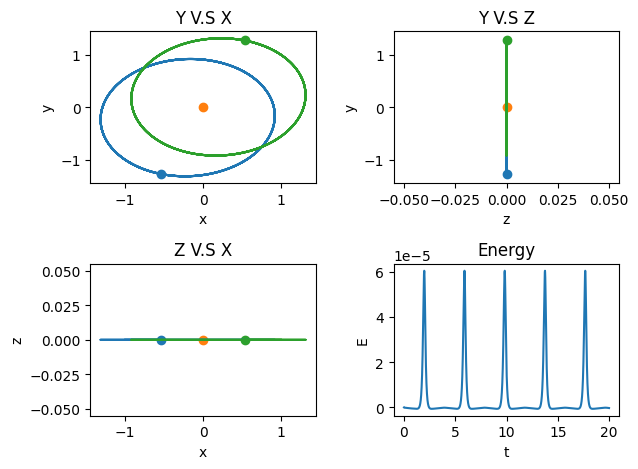
\includegraphics[scale = 0.5]{Conserved_State_1_evolution}
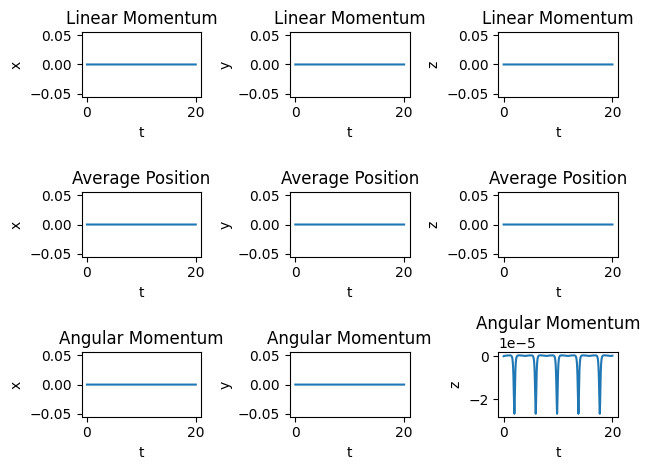
\includegraphics[scale = 0.5]{Conserved_State_1_quantities}
\label{fig:2}\caption{The Conserved evolution and Quantities   [$dt = 0.002, \rho = 0.5, M=100$]}
\end{figure}
\begin{figure}[h]
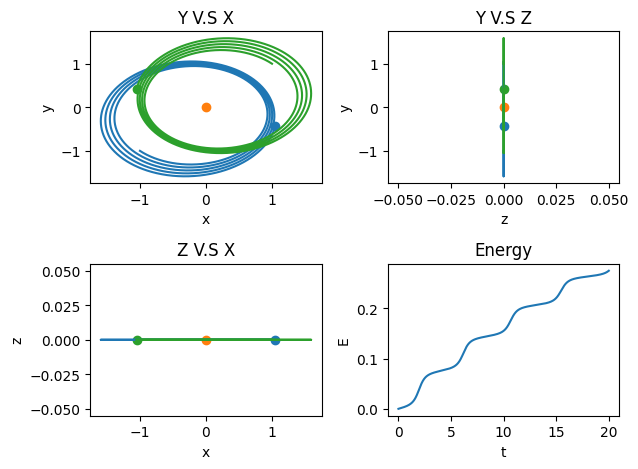
\includegraphics[scale = 0.5]{Unconserved_State_1_evolution}
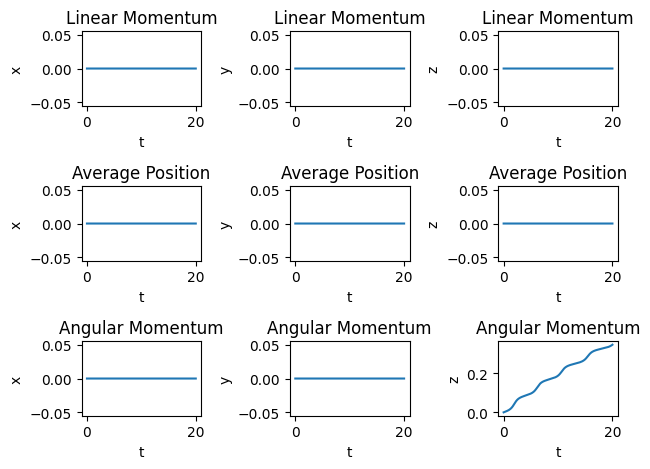
\includegraphics[scale = 0.5]{Unconserved_State_1_quantities}
\label{fig:3}\caption{The Unconserved evolution and Quantities   [$dt = 0.002, \rho = 0.5, M=0$]}
\end{figure}
\end{center}

We now look at a more chaotic state to see how the algorithm fares. This state is given by (insert state here)
%\pagebreak
%Describe setup
%dt=0.0001, \rho = 0.01, M = 10
\begin{center}
\begin{figure}[h]
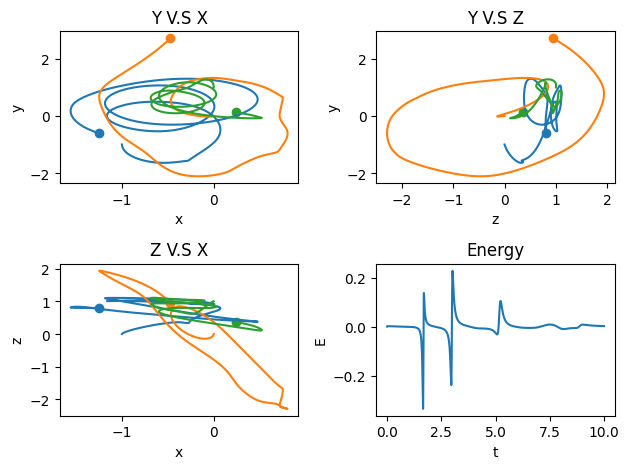
\includegraphics[scale = 0.5]{Conserved_State_2_evolution}
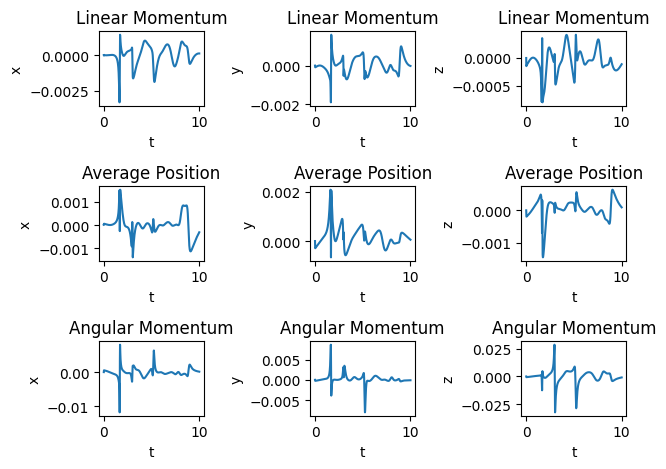
\includegraphics[scale = 0.5]{Conserved_State_2_quantities}
\label{fig:4}\caption{The Conserved evolution and Quantities   [$dt = 0.0001, \rho = 0.01, M=10$]}
\end{figure}
\begin{figure}[h]
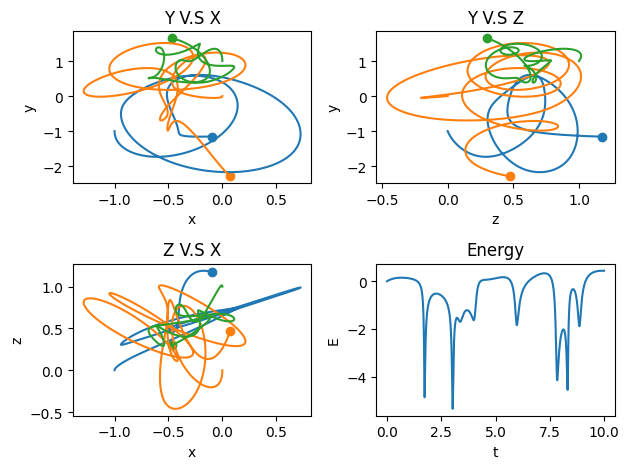
\includegraphics[scale = 0.5]{Unconserved_State_2_evolution}
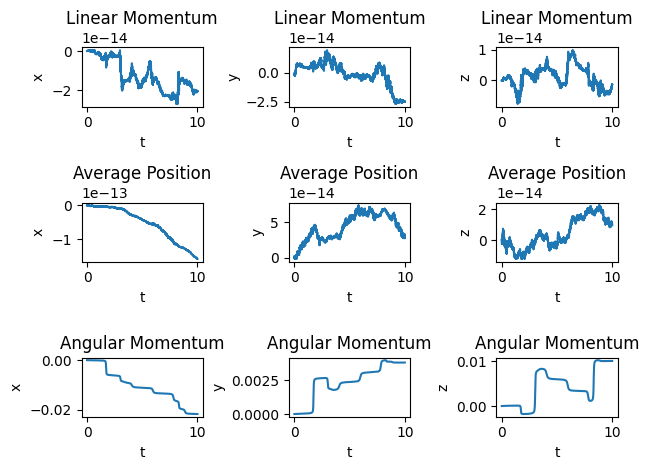
\includegraphics[scale = 0.5]{Unconserved_State_2_quantities}
\label{fig:5}\caption{The Unconserved evolution and Quantities   [$dt = 0.0001, \rho = 0.01, M=0$]}
\end{figure}
\end{center}
\pagebreak

We can compute the eigenvalues over time, for the conserved chaotic state \ref{fig:2}, and we receive the following graphs.	
\begin{center}
\begin{figure}[h]
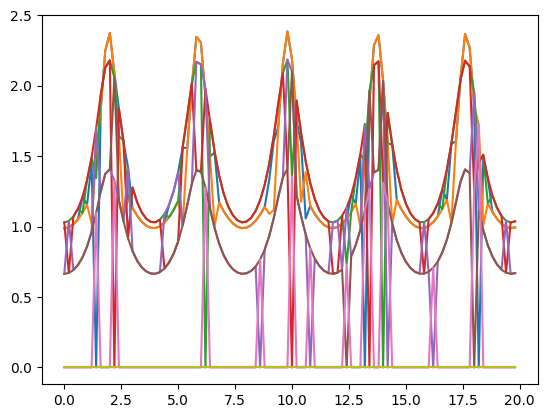
\includegraphics[scale = 0.5]{Conserved_State_1_Eigenvalue_distribution}
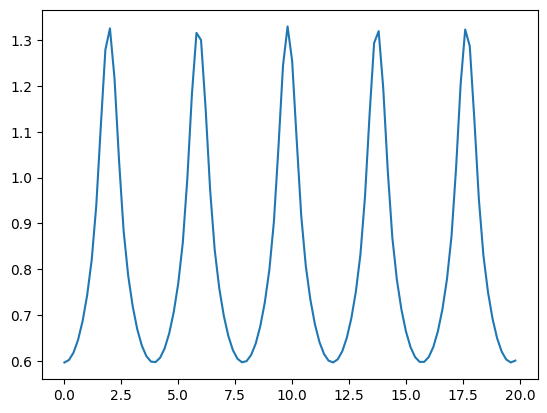
\includegraphics[scale = 0.5]{Conserved_State_1_Eigenvalue_average}
\label{fig:6}\caption{The full eigenvalue spectrum and it's average}
\end{figure}
\end{center}

We can compute the eigenvalues over time, for the conserved chaotic state \ref{fig:4}, and we receive the following graphs.	
\begin{center}
\begin{figure}[h]
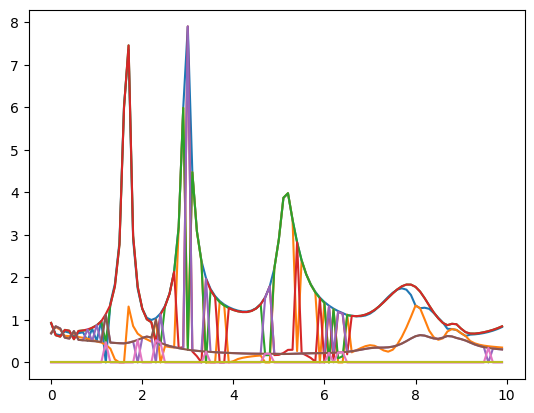
\includegraphics[scale = 0.5]{Conserved_State_2_Eigenvalue_distribution}
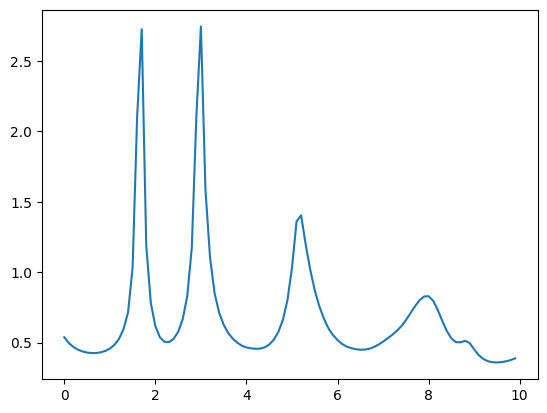
\includegraphics[scale = 0.5]{Conserved_State_2_Eigenvalue_average}
\label{fig:7}\caption{The full eigenvalue spectrum and it's average}
\end{figure}
\end{center}



%Talk about how it just kept not working :(



%Depending on your topic, you might want to show some numerical
%solutions, e.g.~from Maple. If you do this, 
%include a list of the parameter values you are considering (in a table
%if necessary) and say a few words about why you have chosen these
%parameters. You should then present and discuss some figures that
%illustrate the solutions. For clarity, please put your figures at the
%end of the document. You can use labels to link to them. In figure
%\ref{projectile1}, it is clear that the particle range is
%significantly limited when drag is introduced. 


\chapter{Conclusions}

Notice how in figure 6 \ref{fig:6} we see repeated spikes in eigenvalue. This corresponds to an increase in chaos at times $t\approx2, 6, 10, 14, 18$. Notice that the error \ref{fig:2} in all the conserved quantities corresponds with these spikes\\
Also we see that in figure 7 \ref{fig:7} we see three spikes in eigenvalue again. These correspond to an increase in chaos at time $t \approx 2, 3, 5, 8$. Notice that the error \ref{fig:4} in all the conserved quantities corresponds with these spikes\\

Notice that the eigenvalues in the named 'chaotic state' has peaks reaching up to on average $\approx2.6$ where as the 'stable state' has peaks only up to $\approx 1.3$\\

This suggests that in between moments of chaos the state is stable, Generally we see objects move away and are stable and slow but as they speed up they get close together and become less stable\\

One problem with the analysis is that we only calculated the eigenvalues not the eigenvectors. We know that there are always + \& - eigenvalues which in a stable state should cancel. This means that the eigenvectors have to rotate in such a way to oscillate the exponential growth and decay giving stable motion.


%Finally, end with a summary of your problem, approach, and
%findings. It is also nice to finish with some speculation about how
%your results might apply to other problems, and/or to mention avenues
%for future work.


%\begin{figure}
%	\begin{center}
%		%\includegraphics[width=0.7\linewidth]{trajectory1.pdf}
%	\end{center}
%	\caption{Please include informative captions. This figure compares the
%		trajectories of two particles with $m=0.15$ kg and initial velocity
%		30 ms$^{-1}$ oriented 50$^\circ$ from the positive $x$-axis, for a
%		particle with no drag (blue) and quadratic drag with $c=0.001$
%		kgm$^{-1}$ (red).} 
%	\label{projectile1}
%\end{figure}

\chapter{Appendix A: General N-body Problem}
\label{appendix_A}

\epigraph{Mathematics is the art of giving the same name to different things.}{\textit{Henri Poincar\'{e}}}

\section{Relational Setting}

\subsection{States, Configurations and Positions}

Consider a system of $N$ particles with generalized coordinates $\pmb{q}_1, \pmb{q}_2, \dots, \pmb{q}_n \in \mathbb{R}^D$ (usually with $D = 3$), each a function\footnote{Given a \textbf{domain} set $X$ and \textbf{codomain} $Y$, a \textbf{function} will refer to a map $f : X \to Y$ s.t. for all $x \in X$, $\text{im}_f(x) = \{ y \in Y : y = f(x) \}$ is a singleton i.e. every $x \in X$ is assigned exactly one $y \in Y$ under $f$.\label{function_defn}} of time-dependent parameters $\phi_1, \dots, \phi_m \in \mathbb{R}$. It will shortly be explained that by construction, $n \leq N$ and $Dn \leq m$.

The parameters $\phi_1, \dots, \phi_m$ completely describe the state of the system at any given time $t \in \mathbb{R}$. Hence, the set they collectively belong to, say $\mathcal{S}$, will be called the \textbf{state space} of the system. The parameters can be collected together as tuples of the form,

\defn{States}{
$$\hook{\phi}(t) = (\phi_1(t), \dots, \phi_m(t))_\mathcal{S} \in \mathcal{S}$$ 
}
\label{states_defn}

which belong to some region of $\mathbb{R}^m$. Therefore, $\boxed{S \subseteq \mathbb{R}^m}$. The subscript $\mathcal{S}$ denotes that the concerned tuples belong specifically to $\mathcal{S}$ and should not be compared with those in other spaces to be discussed soon.

Similarly, all the generalized coordinates can be collected into tuples in the \textbf{configuration space} Q, so that each collection of generalized coordinates (or 'configuration' of the whole system) resembles,

\defn{Configurations}{
$$\harp{\pmb{q}}(\hook{\phi}(t)) = (\pmb{q}_1(\hook{\phi}(t)), \dots, \pmb{q}_n(\hook{\phi}(t)))_Q \in Q$$
}

and $\boxed{Q \subseteq \mathbb{R}^n}$. 

Last but not the least, the position of each particle is a vector in $\mathbb{R}^D$ and the positions of all $N$ particles are contained in the tuple:

\defn{Positions}{
\begin{align*}
\vec{\rho} = (\pmb{r}_1(\harp{\pmb{q}}(\hook{\phi}(t))), \dots, \pmb{r}_N(\harp{\pmb{q}}(\hook{\phi}(t)))) \in & \: \mathbb{R}^N \times \overset{D \text{ times}}{\dots} \times \mathbb{R}^N \\
& = \mathbb{R}^{DN}
\end{align*}
}
\label{positions_defn}

The above relationships between the concerned quantities and more importantly, the \emph{spaces} they belong to, can be summarized in the form of a commutative diagram,

\begin{figure}[H]
\begin{center}
\begin{tikzcd}
\mathbb{R} \text{ (Time)} \arrow[d, "\vec{\rho} \circ \harp{\pmb{q}} \circ \hook{\phi}" swap] \arrow[rd, "\harp{\pmb{q}} \circ \hook{\phi}"] \arrow[r, "\hook{\phi}"] & \mathcal{S} \text{ (State space)} \arrow[d, "\harp{\pmb{q}}"] \\
\mathbb{R}^{DN} \text{ (Physical space)} & Q \text{ (Configuration space)} \arrow[l, "\vec{\rho}"]
\end{tikzcd}
\end{center}
\caption{Relationships between spaces in which system lives.}
\end{figure}

By the above diagram commuting, we mean that the maps represented by arrows compose as expected i.e. a function from $B \to C$ composed after one from $A \to B$ defines a new function $A \to C$. In other words, the functions in a commutative diagram are transitive under composition and so, going from one set to another (represented by nodes) defines the same function regardless of the path taken. This turns out to follow from the \hyperref[function_defn]{standard definition of functions that we use}.

\newpage
\subsection{Philosophy}

The elements of each of the spaces discussed above tell something about the system. In fact, we imagine that a system \emph{lives} in those spaces, depending on how much information we deem to be 'sufficient' to represent the particles in the system. This depends on the task at hand, which is often one among a set of interlinked problems regarding the nature of the system. 

\rmkb{
In particular, we claim that particles, as far as such problems are concerned, are localized objects and can therefore be represented by time-dependent position vectors (which can be collected into objects like $\vec{\rho}$). \emph{How} these positions change is the subject of \textbf{kinematics}. However, where kinematics, end, \textbf{dynamics} begins, which attempts to explain \emph{why} positions change as they do. 
}

A particular schema for models achieving the task of explaining dynamics is one where a particle has some intrinsic characteristics measured by parameters of the form $\hook{\phi}$, and the way these change with time and interact (perhaps even with the characteristics of other particles) causally explain how the positions of the particles change. Therefore, the question of \emph{why} the particles move as they do can be reframed as \emph{how} the parameters evolve, which by some mechanism set the particles to their expected motion.

One can also take the reverse approach for the above philosophy. We can hold the positions of particles to be the 'fundamental' information representing them, and they have patterns stemming from the dynamics of the system, which can be succinctly contained in convenient parameters.

Either way, there seems to be a multi-layered nature when it comes to the information we want to unravel about a particle, which is why constructs like state space and configuration space are instrumental. Equipped with these thoughts, we will now explain what the said spaces and such constructions physically represent in their philosophical backdrop.

\subsection{Configuration Space}
\label{configuration_space}

Physically, it is perhaps easier to begin with positions and states, and only then move to the more abstract middle ground of configurations, rather than vice-versa.

The positions of particles are Euclidean vectors in a physical i.e. Euclidean space, so they possess magnitude and direction.\footnote{An inner product can be constructed from a norm using the \emph{polarization identity}, thereby endowing the finite-dimensional Euclidean space in question an inner product.} On the other hand, the particles possess parameters at each instant of time that change with its motion in physical space. 

Now, often, particles are \emph{constrained} to move only in a region of a Euclidean space $\mathbb{R}^{DN}$. An example is a body forced to move on a surface. At each moment of time and position in this constrained region of $\mathbb{R}^{DN}$, the particles can move only in a certain number of independent ways, called their \textbf{degrees of freedom}. However, since the constrained region containing the particle is embedded in $\mathbb{R}^{DN}$, \emph{locally}, the degrees of particles the particle can 'seek out' must resemble some lower-dimensional Euclidean space $\mathbb{R}^{Dn}$, so that they can move continuously in independent directions and do other things locally that particles do regardless of constraints. 

\clm{Configuration space as a manifold}{
The space particles are constrained to \emph{is} the configuration space $Q$, and it is only locally required to resemble $\mathbb{R}^{Dn}$ for some $n \leq N$. In general, $Q$ can have a more complicated \emph{global} structure as long as it locally 'looks' Euclidean and these local Euclidean patches 'stitch together' smoothly from point to point. $Q$ is therefore said to be an $Dn$-dimensional \textbf{manifold}.\footnote{Formally, a \emph{manifold} is a topological space in which open neighbourhoods are homeomorphic to some open neighbourhood in some Euclidean space. 

Therefore, regions 'near' each point (encoded in open neighbourhoods) locally 'look' like regions of some Euclidean space and intersections of open neighbourhoods agree up to homeomorphism. When the transition maps between neighbourhoods are $\mathcal{C}^k$, the manifold is said to itself be $\mathcal{C}^k$ i.e. $k$ times differentiable. 

Trivially, any $\mathbb{R}^D$ is a $D$-dimensional manifold with the mentioned bijections and transition maps being identity maps. \\

Here, a \emph{homeomorphism} between topological spaces is a structure-preserving map i.e. it is a continuous bijection that preserves how open neighbourhoods behave via intersections, unions and so forth.}
}

To summarize, while systems of $N$ particles live in physical space $\mathbb{R}^{DN}$, they can be constrained to live on $Dn$-dimensional manifolds (with $n \leq N$) i.e. configuration space $Q$. And for each configuration $\harp{\pmb{q}} \in Q$,\footnote{Each configuration vector $\pmb{q}_m$ lives in the tangent space of $Q$ at some point $q \in Q$ i.e. $\pmb{q}_m \in T_{q} Q$, which can be defined to be the space spanned by the partial derivatives at $q$. The intuition for this is that partial derivatives can be used to build all directional derivatives, the space of which is bijective to the set of all vectors at that point.} the particles have states $\hook{\phi}(\harp{\pmb{q}})$.

\newpage
\section{Some Classifications of Systems}

For future purposes, it is convenient to lay down the definitions for particular kinds of systems, including ones not discussed so far.

\defn{Constrained systems}{
A system of $N$ particles is \textbf{constrained} when its configuration space $Q$ is a proper subset\footnote{up to homeomorphism; we say that a manifold $X$ is a subset of another manifold $Y$ up to homeomorphism if there is a submanifold $S \subseteq Y$ such that $S$ is homeomorphic to $X$.} of the physical space it evolves in i.e. $Q \subsetneq \mathbb{R}^{DN}$ or equivalently, $n < N$.
}

A system that is not constrained is said to be \textbf{non-constrained}. Now, we consider an important aspect of dynamical systems, called \emph{holonomy},

\defn{Holonomic systems}{
A system of $N$ particles is \textbf{holonomic} when its state $\hook{\phi} \in \mathcal{S}$ for a configuration $\harp{\pmb{q}} \in Q$ depends only on the configuration and not the path it took in $Q$ i.e. the state depends only on instantaneous configuration and not the configuration history.
}
\label{holonomy_defn}

\lemp{Dimensional characterization of holonomy}{
A system is holonomic iff $\dim(\mathcal{S}) = \dim(Q)$, i.e., $m = Dn$.
}{
$(\impliedby)$

Suppose for the sake of contradiction that the system concerned is not holonomic i.e. the state $\hook{\phi}$ depends on the path taken to reach a configuration $\harp{\pmb{Q}}$. Then, the following set must have \emph{more} than one element:

$$\preim_{\harp{\pmb{q}}}(\{ \harp{\pmb{Q}} \}) = \left\{ \hook{\Phi} \in \mathcal{S} : \harp{\pmb{q}}(\hook{\Phi}) = \harp{\pmb{Q}} \right\}$$

Therefore, at each configuration $\harp{\pmb{Q}} \in Q$, there are \emph{at least} $2m$ degrees of freedom contained in preimages $\hook{\Phi}_1, \hook{\Phi}_2, \dots, \hook{\Phi}_f \in \mathcal{S} \subseteq \mathbb{R}^{m}$. We can construct a new space $\tilde{\mathcal{S}} \subseteq \mathbb{R}^{mf}$ where $f \geq 2$ so that in this bigger space, the non-injectivity of the state vanishes and there is a 'unique' ensemble of states,

$$\tilde{\Phi} = \left( \hook{\Phi}_1, \hook{\Phi}_2, \dots, \hook{\Phi}_f \right)_{\tilde{\mathcal{S}}} \in \tilde{\mathcal{S}} \subseteq \mathbb{R}^{mf}$$

Hence, we now know that at \emph{each} configuration in $Q$, we can bijectively attach a state from $\tilde{\mathcal{S}}$ which is usually some neighbourhood in some Euclidean space. Therefore, every open neighbourhood in $Q$ 'looks like' the Euclidean space corresponding to $\tilde{\mathcal{S}}$ in the topological sense. This informally suggests that,

$$\dim(Q) = \dim(\tilde{\mathcal{S}})$$

Therefore, we must at least have $\dim(Q) = mf \neq m$. Since $\dim(\mathcal{S}) = m$, it must be the case that when the system is not holonomic, $\dim(Q) \neq \dim(\mathcal{S})$. This is equivalent to the contrapositive implication that when $\dim(Q) \neq \dim(\mathcal{S})$, the system described is holonomic.

$(\implies)$

When a system is holonomic, much like in the above argument, we can attach to each configuration $\harp{\pmb{Q}} \in Q$ a state $\hook{\Phi}$, but by the \hyperref[holonomy_defn]{definition of holonomy}, it must be an instantaneous state and not an ensemble,

$$\left\lvert \preim_{\harp{\pmb{q}}}(\{ \harp{\pmb{Q}} \}) \right\rvert = \left\lvert \left\{ \hook{\Phi} \in \mathcal{S} : \harp{\pmb{q}}(\hook{\Phi}) = \harp{\pmb{Q}} \right\} \right\rvert =1$$

Since $Q$ and $\mathcal{S}$ 'look alike' locally, we now have $\dim(Q) = \dim(\mathcal{S})$. We have thus shown that holonomy implies the said equality, and the converse is true too, which proves the logical equivalence of the two statements.
}  

We define a system to be \textbf{non-holonomic} when it is not holonomic. Equivalently, such systems obey $\dim(Q) \neq \dim(\mathcal{S})$, i.e., $Dn \neq m$. Furthermore, we have the following terminology and equivalent formulation of non-holonomy using it.
\label{non_holonomy_defn}

\label{loop_defn}
\defn{Loop}{
A \textbf{loop} in a topological space $X$ is a continuous curve $\Gamma : [0, 1] \to X$ with $\Gamma(0) = \Gamma(1)$. \\

Equivalently, via continuous maps $\lambda : \mathbb{R} \to [0, 1]$, a loop is a curve $\gamma = \Gamma \circ \lambda : \mathbb{R} \to M$ such that there exists a $T \in \mathbb{R}$ such that $\gamma(t) = \gamma(t + nT)$ for all $t \in \mathbb{R}, n \in \mathbb{Z}$. \footnote{Another way of saying this is that $\gamma$ can be \emph{identified} after every so-called time period $T$.}
}

\clmp{Loops as continuous deformations of $S^1$}{
continuous maps $\varphi$ from the \emph{unit circle} $S^1 = \{ (x, y) \in \mathbb{R}^2 : x^2 + y^2 = 1 \}$ to $X$ sufficiently characterize loops.
}{
Let $\xi : [0, 1] \to S^1$ be the periodic, continuous map $\xi(\lambda) = (\cos(\lambda), \sin(\lambda))$. Hence, $\gamma = \varphi \circ \xi : [0, 1] \to X$ is a continuous map with $\gamma(0) = \gamma(1)$ i.e. a loop.
}

\begin{figure}[H]
\begin{center}
\begin{tikzcd}
\mathbb{R} \arrow[r, "\lambda"] & X \\
{[0, 1]} \arrow[u, "\Gamma"] \arrow[ru, "\gamma"] \arrow[r, "\xi"] & S^1 \arrow[u, "\varphi"]
\end{tikzcd}
\caption{Loops in a topological space $X$ defined using various spaces.}
\end{center}
\end{figure}

\newpage
\thmr{Loop characterization of non-holonomy}{loop_characterization_non_holonomy}{
A system is non-holonomic iff there exists a loop $C$ in the configuration space $\mathcal{Q}$ such that the system's state changes (by a non-zero amount) when it traverses a full cycle along the loop.
}

\pf{
($\impliedby$)

Consider the closed loop $C$ described above. If the system starts at a coonfiguration $\harp{\pmb{q}}$ with state $\hook{\phi}_0$ and traverses along the loop, \hyperref[loop_defn]{by definition}, the configuration returns to $\harp{\pmb{q}}$ and yet, by construction, the final state $\hook{\phi}_1 \neq \hook{\phi}_0$. Hence, the state $\hook{\phi}$ depends on the history of the curve traversed to reach the concerned configuration $\harp{\pmb{q}}$. \hyperref[non_holonomy_defn]{By definition}, the system is non-holonomic. We can extend the above observation to $n$ cycles of traversal along $C$, giving rise to potentially different states $\hook{\phi}_n$. This is a special case of a loop space consideration we will construct in the next subsection.

($\implies$)

Let the system in question be non-holonomic as defined earlier. Let $\gamma_1, \gamma_2 \in \mathcal{C}(\mathbb{R}, \mathcal{Q}) = \mathcal{Q}^{\mathbb{R}} \cap C(\mathbb{R})$ be distinct continuous curves\footnote{The notation $B^A$ denotes the space of all functions $f : A \to B$ which is an abuse of notation based on the fact that the cardinality of $B^A$ is, in fact, $|B|^{|A|}$. \\

Therefore, $B^A \cap C^n(A)$ denotes the space of all k-times differentiable functions $A \to B$, for which we choose the alternative notation $\mathcal{C}^k(A, B)$.} from a configuration $\harp{\pmb{q}}_1 \in \mathcal{Q}$ to another configuration $\harp{\pmb{q}}_2 \in \mathcal{Q}$. Equivalently, using a continuous map $t : [0, 1] \to \mathbb{R}$, we have curves $\Gamma_1, \Gamma_2$ defined using $\Gamma_i = \gamma_i \circ t$, such that $\gamma_i(0) = \harp{\pmb{q}}_1, \gamma_i(1) = \harp{\pmb{q}}_2$ for $i = 1, 2$. Non-holonomy guaruntees that there exists such a pair of curves with the same endpoints such that,

\begin{align*}
\int_{\gamma_1} d \hook{\phi} & \neq \int_{\gamma_2} d \hook{\phi} \\
\int_{\gamma_1} d \hook{\phi} - \int_{\gamma_2} d \hook{\phi} & \neq \hook{0}
\end{align*}

Let us formally define the 'reverse' of a curve as follows:

$$\tilde{\Gamma}_i : \begin{cases}
[0, 1] & \to \mathcal{Q} \\
\lambda & \mapsto \Gamma_i(1 - \lambda)
\end{cases}$$

Correspondingly,

$$\tilde{\gamma}_i : \begin{cases}
\mathbb{R} & \to \mathcal{Q} \\
t & \mapsto \gamma_i(t_2 - t)
\end{cases}$$

where $\gamma_i(t_2) = \harp{\pmb{q}}_2$. 

By the fundamental theorem of calculus, interchanging the limits of an integral, or equivalently, reversing the curve of intergation, reverses the signature of the said integral\footnote{As a corollary, even in a non-holonomic situation, it is guarunteed that loops of the form $\tilde{\gamma} * \gamma$ bring back the state $\hook{\phi}$ to its original value as the changes are cancelled out by the first traversal and then its retrograde version.}. Hence,

$$\int_{\tilde{\gamma}_i} d \hook{\phi} = - \int_{\gamma_i} d \hook{\phi}$$

Substituting this into the second term of the first relation we derived from non-holonomy above, we find,

$$\int_{\gamma_1} d \hook{\phi} + \int_{\tilde{\gamma}_2} d \hook{\phi} \neq \hook{0}$$

But the above integration is the same as along the concatenation of the paths $\gamma_1$ and $\tilde{\gamma}_2$ i.e. the loop $\tilde{\gamma}_2 * \gamma_1$ where concatenation $* : \mathcal{C}(\mathbb{R}, \mathcal{Q}) \times \mathcal{C}(\mathbb{R}, \mathcal{Q}) \to \mathcal{C}(\mathbb{R}, \mathcal{Q})$ is defined by,
\label{concatenation}

$$(\Gamma_2 \textcircled{$*$} \Gamma_1)(\lambda) = \begin{cases}
\Gamma_1(2 \lambda) & \lambda \in \left[ 0, \frac{1}{2} \right] \\
\Gamma_2(2 \lambda - 1) & \lambda \in \left[ \frac{1}{2}, 1 \right]
\end{cases}$$

By construction we must have, $\Gamma_1(1) = \Gamma_2(0)$. Thus, $\Gamma_2$ has been 'stitched' to the end of $\Gamma_1$ in a continuous manner. Correspondingly,

\begin{align*}
\tilde{\gamma}_2 * \gamma_1 & = (\tilde{\gamma}_2 \textcircled{$*$} \Gamma_1) \circ \lambda \\
& = \begin{cases}
\gamma_1(2t) & t \in \left[ t_1, \frac{t_2 - t_1}{2} \right] \\
\tilde{\gamma}_2(2t - t_1) & t \in \left[ \frac{t_2 - t_1}{2}, t_2 \right]
\end{cases}
\end{align*}

with $\gamma_1(t_2) = \tilde{\gamma}_2(t_1)$, which is valid since by construction $\gamma_1(t_2) = \tilde{\gamma}_2(t_1) = \harp{\pmb{q}}_2$. 

The key takeaway from the above discussion is that curves can be concatenated and this corresponds to the addition of integrals along them\footnote{These notions indicate that path reversal is like an inverse operation and the paths themselves look like groups with a concatenation operation, which leads to structures such as homotopy groups and the larger discipline of algebraic topology.},

\begin{align*}
\oint_{\tilde{\gamma}_2 * \gamma_1} d \hook{\phi} & = \int_{\gamma_1} d \hook{\phi} + \int_{\tilde{\gamma}_2} d \hook{\phi} \\
& \neq \hook{0}
\end{align*}

Therefore, non-holonomy implies the existence of loops along which states can change. This completes the proof that non-holonomy is equivalent to this property of state change over closed paths in $\mathcal{Q}$.
}

\cor{
A system is holonomic iff for every loop $\gamma : \mathbb{R} \to \mathcal{Q}$, traversal along it does not change the state $\hook{\phi}$ i.e.,

$$\oint_{\gamma} d \hook{\phi} = \hook{0}$$
}

Below are some diagrams which depict the kinds of concatenation mentioned above.

\begin{figure}[H]
\begin{center}
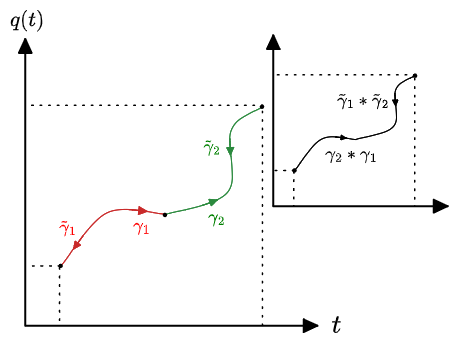
\includegraphics[scale=0.6]{concat_curve} 
\caption{A one-dimensional representation of curves and their reversals and concatenations}
\end{center}
\end{figure}

\begin{figure}[H]
\begin{center}
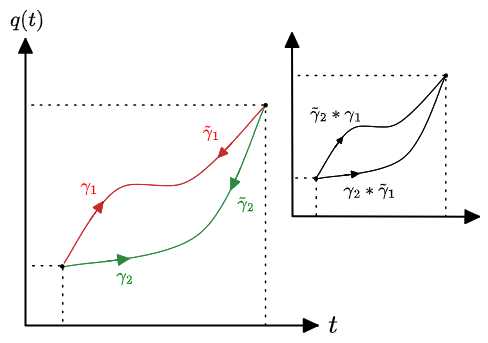
\includegraphics[scale=0.6]{concat_loop} 
\caption{Concatenating curves with fixed enpoints generates loops.}
\end{center}
\end{figure}

\newpage
\section{Loop Spaces}
\label{loop_spaces}

\subsection{Based, Unbased and Free Loop Spaces}

To formalize the notion of 'every loop', we define loop spaces.

\defn{(Based) loop space}{
The \textbf{based loop space} or simply, \textbf{loop space} $\mathscr{L}_{\harp{\pmb{q}}}$ at a configuration $\harp{\pmb{q}} \in \mathcal{Q}$ is a map $\mathcal{Q} \to \mathcal{C}([0, 1], \mathcal{Q})$ such that,

$$\mathscr{L}_{\harp{\pmb{q}}} = \left\{ \gamma \in \mathcal{C}([0, 1], \mathcal{Q}) : \gamma(0) = \gamma(1) = \harp{\pmb{q}} \right\}$$
}

A loop space in which the identified endpoints of loops are not restricted to be a base configuration, so that any point in the loop can be the base configuration, is called an unbased loop space at that configuration, 

\defn{Unbased loop space}{
The \textbf{unbased loop space} $\mathcal{L}_{\harp{\pmb{q}}}$ at a configuration $\harp{\pmb{q}} \in \mathcal{Q}$ is a map $\mathcal{Q} \to \mathcal{C}([0, 1], \mathcal{Q})$ defined as,

$$\mathcal{L}_{\harp{\pmb{q}}} = \left\{ \gamma \in \mathcal{C}([0, 1], \mathcal{Q}) : \gamma(0) = \gamma(1), \harp{\pmb{q}} \in \gamma \right\}$$
}

Trivially, every based loop space is a subset of a corresponding unbased loop space. These notions become equivalent under translation equivalence in the parameter space $[0, 1]$ since such translations 'turn' a loop around to set the identified endpoint $\gamma(0) = \gamma(1)$ to be the base configuration $\harp{\pmb{q}}$.

The loop spaces at all points in the configuration space can be collected together into a free loop space,

\defn{Free loop space}{
The \textbf{free} or \textbf{total loop space} $\Omega \mathcal{Q}$ is the union of loop spaces of all configurations,

$$\Omega \mathcal{Q} = \underset{\harp{\pmb{q} \in \mathcal{Q}}}{\bigcup} \mathscr{L}_{\harp{\pmb{q}}} = \left\{ \gamma \in \mathcal{C}([0, 1], \mathcal{Q}) : \gamma(0) = \gamma(1) \right\}$$
}

It can be shown that the free loop spaces for based and unbased loops are equal. This is because every unbased loop passing through a configuration is a based loop in some other loop space and vice-versa, so collecting all loops together does not 'remember' if they were based or unbased.

\newpage
Starting with the free loop space, one can construct unbased and then based loop spaces using projections, which are defined as follows,

\defn{Projection}{
A projection from a set $A$ to a subset $U$ is a surjection $\pi : A \to U$ such that $\pi$ is idempotent, i.e., $\pi \circ \pi = \id_{U}$. 

If $A$ is a topological space\footnote{$U$ would then be equipped with the subset topology with respect to that of $A$.}, $\pi$ is also continuous. 
}

Intuitively, a projection projects a space down to a subspace and destroys as much information in the process as possible, so that applying the projection again has no incremental effect. It trivially follows from the definitions of the various \hyperref[loop_spaces]{loop spaces} listed above that they can be projected into one another:

\clm{Loop space projections}{
\begin{enumerate}
\item $\Omega \mathcal{Q} \overset{\pi_{\harp{\pmb{q}}}}{\rightarrow} \mathcal{L}_{\harp{\pmb{q}}}$ where,

$$\pi_{\harp{\pmb{q}}}(\Omega \mathcal{Q}) = \left\{ \gamma \in \Omega \mathcal{Q} : \harp{\pmb{q}} \in \gamma \right\} = \mathcal{L}_{\harp{\pmb{q}}}$$

\item $\mathcal{L}_{\harp{\pmb{q}}} \overset{\pi}{\rightarrow} \mathscr{L}_{\harp{\pmb{q}}}$ with,

$$\pi(\mathcal{L}_{\harp{\pmb{q}}}) = \left\{ \gamma \in \mathcal{L}_{\harp{\pmb{q}}} : \gamma(0) = \harp{\pmb{q}} \right\} = \mathscr{L}_{\harp{\pmb{q}}}$$
\end{enumerate}
}

Therefore, building 'up' from based loop spaces to unbased and free ones is equivalent to building 'down' in the reverse order. When loop spaces are equipped with topologies, $(\Omega \mathcal{Q}, \pi_{\harp{\pmb{q}}}, \mathcal{L}_{\harp{\pmb{q}}})$ and $(\mathcal{L}_{\harp{\pmb{q}}}, \pi, \mathscr{L}_{\harp{\pmb{q}}})$ become bundles.\footnote{Given a continuous projection $\pi : A \to U$, a \textbf{bundle} is the triplet $(A, \pi, U)$ where $A$ is called the \textbf{total space} and $U$ is the \textbf{base space}. Over every $p \in U$ lives a corresponding \textbf{fibre}, defined as $F_p = \preim_{\pi}(\{ p \})$. \\ 

For the bundles described with regard to loop spaces, when the total space is the free loop space $\Omega \mathcal{Q}$, the fibre over each unbased loop $\gamma \in \mathcal{L}_{\harp{\pmb{q}}}$ is $F_{\gamma} = \left\{ \delta \in \Omega \mathcal{Q} : \harp{\pmb{q}} \in \delta \implies \delta = \gamma \right\} = \mathcal{L}_{\harp{\pmb{q}}}$ i.e. every fibre is identically the unbased loop space. We thus say that $(\Omega \mathcal{Q}, \pi_{\harp{\pmb{q}}}, \mathcal{L}_{\harp{\pmb{q}}})$ is a \textbf{fibre bundle} with a \textbf{typical fibre} $F = \mathcal{L}_{\harp{\pmb{q}}}$.

Similarly, when an unbased loop space $\mathcal{L}_{\harp{\pmb{q}}}$ is the total space, the fibre living on a based loop $\gamma \in \mathscr{L}_{\harp{\pmb{q}}}$ is $F_{\gamma} = \left\{ \delta \in \mathcal{L}_{\harp{\pmb{q}}} : \delta(0) = \harp{\pmb{q}} \implies \delta = \gamma \right\} = \mathscr{L}_{\harp{\pmb{q}}}$. Therefore, once again, $(\mathcal{L}_{\harp{\pmb{q}}}, \pi, \mathscr{L}_{\harp{\pmb{q}}})$ is a fibre bundle with the typical fibre being the based loop space. 

These notions formalize the idea of unbased/based loop spaces 'living on' the unbased/based loops in them. Since unbased/based loops correspond in a one-to-one manner with the configurations in them/endpoint configurations respectively, we can also construct appropriate bundles with loop spaces living over the configuration space.\label{loop_bundles}}

With these ideas in mind, we can formally revisit the concatenation of loops.

\subsection{Concatenation}

\defn{Concatenation}{
Concatenation $* : \mathscr{L}_{\harp{\pmb{q}}} \times \mathscr{L}_{\harp{\pmb{q}}} \to \mathscr{L}_{\harp{\pmb{q}}}$ is the operation:

$$\gamma_2 * \gamma_1 = \begin{cases}
\gamma_1(2 \lambda) & \lambda \in \left[ 0, \frac{1}{2} \right] \\
\gamma_2(2 \lambda - 1) & \lambda \in \left[ \frac{1}{2}, 1 \right]
\end{cases}$$
}

Since every based loop is an unbased loop, we can extend concatenation similarly to unbased loop spaces. The mathematical significance of concatenation is that it helps form a group,

\clm{$(\mathscr{L}_{\harp{\pmb{q}}}, *)$ as a non-Abelian group}{
\begin{itemize}
\item It can be verified that $(\mathscr{L}_{\harp{\pmb{q}}}, *)$ is a group since it obeys the \textbf{group axioms}:

\begin{enumerate}
\item $\mathscr{L}_{\harp{\pmb{q}}}$ is \textbf{closed} under $*$ i.e.,

$$\forall \gamma_1, \gamma_2 \in \mathscr{L}_{\harp{\pmb{q}}} : \gamma_2 * \gamma_1 \in \mathscr{L}_{\harp{\pmb{q}}}$$

\item $*$ is \textbf{associative},

$$\forall \gamma_1, \gamma_2, \gamma_3 \in \mathscr{L}_{\harp{\pmb{q}}} : \gamma_3 * (\gamma_2 * \gamma_1) = (\gamma_3 * \gamma_2) * \gamma_1$$

\item There is an \textbf{identity} or \emph{constant loop} $\gamma_e \in \mathscr{L}_{\harp{\pmb{q}}}$,

$$\forall \gamma \in \mathscr{L}_{\harp{\pmb{q}}} : \gamma_e * \gamma = \gamma * \gamma_e = \gamma$$

where $\gamma_e(\lambda) = \harp{\pmb{q}}$.

\item Every loop $\gamma \in \mathscr{L}_{\harp{\pmb{q}}}$ has an \textbf{inverse} $\tilde{\gamma} \in \mathscr{L}_{\harp{\pmb{q}}}$ (the same as \emph{reversed} loops),

$$\forall \gamma \in \mathscr{L}_{\harp{\pmb{q}}} : \exists \: \tilde{\gamma} \in \mathscr{L}_{\harp{\pmb{q}}} : \tilde{\gamma} * \gamma = \gamma * \tilde{\gamma} = \gamma_e$$
\end{enumerate}

\item $(\mathscr{L}_{\harp{\pmb{q}}}, *)$ is a \textbf{non-Abelian} group as $*$ is \textbf{non-commutative}, i.e,

\qquad \qquad \qquad \qquad \qquad \quad $\gamma_1, \gamma_2 \in \mathscr{L}_{\harp{\pmb{q}}} \slashed{\implies} \gamma_1 * \gamma_2 = \gamma_2 * \gamma_1$
\end{itemize}
}

Due to the above facts, concatenation provides an algebraic structure to loops, which are geometric objects. This allows one to treat the loops in a way in which they algebraically encode topological information about the configuration space $\mathcal{Q}$, such as how many holes it may have. Such notions are the subject of topological invariants, homotopy theory and algebraic topology in general. 

Now that we have seen how loops come up in holonomy theory and how they lead to various disciplines, let us return to their role in the study of non-holonomic systems in classical mechanics. 

\subsection{Relationship With State Spaces}

Recall that for non-holonomic systems, states $\hook{\phi}$ cannot be uniquely characterized by configurations $\harp{\pmb{q}}$ as new states can be generated at the same configuration by making the system travel along loops $C \in \mathscr{L}_{\harp{\pmb{q}}}$. But this also means:

\thm{Isomorphism of state and loop spaces}{
The state space at a configuration $\harp{\pmb{Q}} \in \mathcal{Q}$ is isomorphic to the associated based loop space $\mathscr{L}_{\harp{\pmb{Q}}}$,

\begin{align*}
\preim_{\harp{\pmb{q}}}(\{ \harp{\pmb{Q}} \}) & = \left\{ \hook{\Phi} \in \mathcal{S} : \harp{\pmb{q}}(\hook{\Phi}) = \harp{\pmb{Q}} \right\} \\
& = \left\{ \oint_{\gamma \in \mathscr{L}_{\harp{\pmb{Q}}}} d \hook{\pmb{\psi}} : \hook{\pmb{\psi}} \in \mathcal{S} \right\} \cong \mathscr{L}_{\harp{\pmb{Q}}}
\end{align*}
}

\pf{
From the equation part of the above statement, we can glean that since every state at a configuration is specified by some based loop, the state space at the configuration must be a subset of the based loop space, up to isomorphism.

But no two distinct based loops $\gamma_1, \gamma_2$ generate the same state since if they did, one could traverse along $\tilde{\gamma}_2 * \gamma_1$ and not change the state, so this concatenated loop must be the constant loop $\gamma_e = \harp{\pmb{Q}}$ which is not necessary (in fact, it only happens when $\gamma_1 = \gamma_2$). Hence, the based loop space is a subset of the state space up to isomorphism.

The two situations above prove the claim.
}

The intuition for the above statement is that every distinct based loop at a configuration generates a distinct state, and since there are no other variables involved, the only states at the configuration are those generated by loops in this manner. As a result, the entire state space is bijective to the free loop space.

\newpage
\cor{
The state space $\mathcal{S}$ is isomorphic to the free loop space $\Omega \mathcal{Q}$ associated with the configuration space $\mathcal{Q}$,

$$\mathcal{S} = \preim_{\harp{\pmb{q}}}(\mathcal{Q}) \cong \Omega \mathcal{Q}$$
}

\pf{
We have,

\begin{align*}
\preim_{\harp{\pmb{q}}}(\mathcal{Q}) & = \preim_{\harp{\pmb{q}}}\left( \underset{\harp{\pmb{Q}} \in \mathcal{Q}}{\bigcup} \{ \harp{\pmb{Q}} \} \right) \\
& = \underset{\harp{\pmb{Q}} \in \mathcal{Q}}{\bigcup} \preim_{\harp{\pmb{q}}}(\{ \harp{\pmb{Q}} \}) \\
& \cong \underset{\harp{\pmb{Q}} \in \mathcal{Q}}{\bigcup} \mathscr{L}_{\harp{\pmb{Q}}} = \Omega \mathcal{Q}
\end{align*}
}

\textbf{Therefore, loops not only unite topological and algebraic aspects of manifolds such as $\mathcal{Q}$, but also provide a description of the state space $\mathcal{S}$ living on the configuration space}! This also means that states in any physical system can be represented by loops, which can be extended into extensive formalisms such as Wilson loops in field theory and spin networks in loop quantum gravity.

In fact, \textbf{the loop space consideration formalizes what it means for the state space to 'live on' the configuration space in the first place}, via topological bundles. In footnote \ref{loop_bundles}, we have shown how loop spaces and their projections define bundles. We can consider this for the collection of all loop spaces i.e. the free loop space $\Omega \mathcal{Q}$ and find that:

\clm{State and configuration spaces form bundles}{
$(\Omega \mathcal{Q}, \Pi, \mathcal{Q})$ is a bundle where the projection $\Pi : \Omega \mathcal{Q} \to \mathcal{Q}$ is defined by,

\begin{align*}
\Pi_{\harp{\pmb{q}}} & = \pi_{\harp{\pmb{q}}} \circ \pi \circ \sigma \\
\Pi(\Omega \mathcal{Q}) & = \left\{ \Pi_{\harp{\pmb{q}}}(\Omega \mathcal{Q}) : \harp{\pmb{q}} \in \mathcal{Q} \right\} = \mathcal{Q}
\end{align*}

where,

$$\{ \sigma(\harp{\pmb{q}}) \} = \left\{ \gamma(0) : \gamma \in \mathscr{L}_{\harp{\pmb{q}}} \right\}$$

i.e., $\sigma(\harp{\pmb{q}}) = \gamma(0)$ for any $\gamma \in \mathscr{L}_{\harp{\pmb{q}}}$.}

All the maps involved above are projections, therefore so are their compositions and unions over subspaces, implying that $\Pi$ is a projection.

Pictorially, the above mechanism can be represented using the commutative diagram below:

\begin{figure}[H]
\begin{center}
\begin{tikzcd}
\Omega \mathcal{Q} \arrow[d, bend right, "\varphi^{-1}" swap] \arrow[rrd, "\Pi_{\harp{\pmb{q}}}" swap] \arrow[r, "\pi_{\harp{\pmb{q}}}"] & \mathcal{L}_{\harp{\pmb{q}}} \arrow[r, "\pi"] & \mathscr{L}_{\harp{\pmb{q}}} \arrow[d, "\sigma"] \\
\mathcal{S} \arrow[u, bend right, "\varphi" swap] \arrow[rr, "\Pi_{\harp{\pmb{q}}} \circ \varphi" swap] & & \harp{\pmb{q}}
\end{tikzcd}
\end{center}
\caption{Projections between loop spaces and the configuration space, as well as the isomorphism of the free loop space and the state space. All the arrows with their nodes in this diagram are bundles.}
\end{figure}

But since $\Omega \mathcal{Q} \cong \mathcal{S}$, there exists a homeomorphism $\varphi : \mathcal{S} \to \Omega \mathcal{Q}$. Therefore, $(\Omega \mathcal{Q}, \Pi, \mathcal{Q})$ being a bundle also implies that $(\mathcal{S}, \Pi \circ \varphi, \mathcal{Q})$ is a bundle. Thus, \textbf{states live over configurations in a concrete topological sense!}

\subsection{Philosophy}

The reasons we discussed the above coming together of various ideas somewhat elaborately are as follows:

\begin{enumerate}
\item The above kind of framework, which forms the basis of \textbf{non-holonomic mechanics}, lays a foundation for studying the theoretical mechanics of systems exhibiting non-holonomy as well as the subclass of systems where non-holonomy disappears i.e. holonomic systems.

\item The general N-body problem involves \textbf{collisions}, in which \hyperref[avoiding_collisions]{non-holonomy plays a fundamental role}.

\item \textbf{Periodic solutions} in N-body problems are $C^2$ loops in configuration space, therefore topological notions to do with them, such as the \textbf{stability} of their perturbations, involve algebraic topology.
\end{enumerate}

\newpage
\section{Constraints}

\subsection{Classification}

A constraint is a relationship between the generalized coordinates and potentially, its derivatives, that may have the effect of restricting a system to a submanifold of the ambient Euclidean space (although this is uncommon for velocity-dependent constraints).

A constraint only involving generalized position and time, but no derivatives of the former, is said to be holonomic,

\defn{Holonomic constraint}{
A \textbf{holonomic constraint} is a relationship involving a function $f : \mathcal{Q} \times \mathbb{R} \to \mathbb{R}$ such that,

$$f(\harp{\pmb{q}}, t) = 0$$
}
\label{holonomic_constraint_defn}

A constraint that does \emph{not} involve time is called \textbf{scleronomous}. Constraints that, on the other hand, involve time, are said to be \textbf{rheonomous}. A constraint that cannot be written in the holonomic form is called a \textbf{non-holonomic constraint}. 

\rmkb{A system having a holonomic constraint does \emph{not} imply that it is holonomic, but nonetheless enables us to test if it is holonomic, as we will see.}

Two important generalizations of holonomic constraints are those of semi-holonomic and Pfaffian constraints.

\defn{Semi-holonomic constraint}{
A \textbf{semi-holonomic} or \textbf{velocity-dependent constraint} is one which can be written, using some map $f : \mathcal{Q} \times T \mathcal{Q} \times \mathbb{R}$, as:

$$f \left( \harp{\pmb{q}}, \frac{d \harp{\pmb{q}}}{dt}, t \right) = 0$$
}
\label{semi_holonomic_constraint_defn}

\newpage
It will be shown that semi-holonomic constraints are further generalized by Pfaffian constraints, 

\defn{Pfaffian constraint}{
A \textbf{Pfaffian} or \textbf{semi-holonomic constraint} is one which can be written in the form,

$$A(d \harp{\pmb{q}}) + A_t dt = 0$$

where the quantity on the left hand side is the \textbf{Pfaffian form} applied to tangent vectors of $\mathcal{Q}$ as well as differentials of time,

\begin{align*}
A(d \harp{\pmb{q}}) + A_t dt & = \sum_{\alpha=1}^{n} A_\alpha (d \pmb{q}_\alpha) + A_t dt \\
& = \sum_{\alpha=1}^{n} A_\alpha \left( \sum_{i=1}^{f} dq_{\alpha i} \pmb{e}_i \right) + A_t dt \\
& = \sum_{\alpha=1}^{n} \sum_{i=1}^{f} dq_{\alpha i} A_\alpha \left( \pmb{e}_i \right) + A_t dt \\
& = \sum_{\alpha=1}^{n} \sum_{i=1}^{f} A_{\alpha i} dq_{\alpha i} + A_t dt \\
& = A_{\alpha i} dq^{\alpha i} + A_t dt & [= 0]
\end{align*}
}

In the last line above, we have used the Einstein summation convention where dummy indices (pairs of identical upper and lower indices) imply summation over them. The object $A$ is a collection of 1-forms $A_{\alpha}$ i.e. linear maps $A_\alpha : T_q \mathcal{Q} \to \mathbb{R}$ and $A_t$ is a 0-form i.e. a scalar.

\newpage
\lemp{Semi-holonomic constraints are Pfaffian}{
All semi-holonomic constraints are Pfaffian.
}{
\begin{align*}
f \left( \harp{\pmb{q}}, \frac{d \harp{\pmb{q}}}{dt}, t \right) & = 0 \\
f(\pmb{q}^1, \dots, \pmb{q}^n, \dot{\pmb{q}}^1, \dots, \dot{\pmb{q}}^n, t) & = 0 \\
f(q^{1 1}, \dots, q^{1 f}, \dots, q^{n 1}, \dots, q^{n f}, \dot{q}^{1 1}, \dots, \dot{q}^{1 f}, \dots, \dot{q}^{n 1}, \dots, \dot{q}^{n f}, t) & = 0
\end{align*}

Let $f$ in summation limits denote $\dim(\mathcal{Q})$. Now, we can take the differential of the above equation to find, using the multivariable chain rule and the Einstein summation convention,

\begin{align*}
df & = 0 \\
\frac{\partial f}{\partial q^{\alpha i}} dq^{\alpha i} + \frac{\partial f}{\partial \dot{q}^{\alpha i}} d \dot{q}^{\alpha i} + \frac{\partial f}{\partial t} dt & = 0 \\
\frac{\partial f}{\partial q^{\alpha i}} dq^{\alpha i} + \frac{\partial f}{\partial \dot{q}^{\alpha i}} \frac{d \dot{q}^{\alpha i}}{dt} dt + \frac{\partial f}{\partial t} dt & = 0 \\
\frac{\partial f}{\partial q^{\alpha i}} dq^{\alpha i} + \left( \frac{\partial f}{\partial \dot{q}^{\alpha i}} \ddot{q}^{\alpha i} + \frac{\partial f}{\partial t} \right) dt & = 0
\end{align*}

Plugging in the Pfaffian constraint,

$$\frac{\partial f}{\partial q^{\alpha i}} dq^{\alpha i} + \left( \frac{\partial f}{\partial \dot{q}^{\alpha i}} \ddot{q}^{\alpha i} + \frac{\partial f}{\partial t} \right) dt = A_{\alpha i} dq^{\alpha i} + A_t dt$$

By multilinearity,

\begin{align*}
A_{\alpha i} & = \frac{\partial f}{\partial q^{\alpha i}} \\
A_t & = \frac{\partial f}{\partial \dot{q}^{\alpha i}} \ddot{q}^{\alpha i} + \frac{\partial f}{\partial t}
\end{align*}

\newpage
In coordinate-free language, we can write the spacelike part of the Pfaffian form at a configuration $\harp{\pmb{q}} \in \mathcal{Q}$ in terms of the gradient of $f$ at that point,

$$A = \dif f$$

But from the semi-holonomic constraint, we have $\dif f = 0$. Hence, $A = 0$, which is a Pfaffian constraint.
}

Furthermore, all holonomic constraints are trivially semi-holonomic constraints involving vanishing functions $f : \mathcal{Q} \times T \mathcal{Q} \times \mathbb{R} \to \mathbb{R}$ that do not explicitly depend on generalized velocity. But since semi-holonomic constraints are Pfaffian, so are holonomic constraints.

\newpage
\subsection{Homotopic Notions}

The above principles can be extended to find when a Pfaffian constraint is semi-holonomic.

\lem{Poincar\'{e}'s lemma}{
Let the configuration space $\mathcal{Q}$ be a \emph{contractible manifold}. This is a sufficient condition for the Pfaffian form $A$ being closed (i.e. $\dif A = 0$, which follows from the Pfaffian constraint $A = 0$) to imply that it is exact i.e. there is a function $f : \mathcal{Q} \times T \mathcal{Q} \times \mathbb{R} \to \mathbb{R}$ such that $A = \dif f = 0$, which is a semi-holonomic constraint.\footnote{Moreover, if $A$ does not explicitly depend on generalized velocity, the constraint is holonomic.}

The above statement, equivalent to \textbf{Poincar\'{e}'s lemma}, says, in other words, that every Pfaffian constraint is semi-holonomic if\footnote{not to be confused with \emph{if and only if}.} $\mathcal{Q}$ is contractible.
}

Proving Poincar\'{e}'s lemma, and in fact, defining contractible manifolds, relies on homotopy theory. In this subsection, we will briefly describe certain aspects of the theory and see what they entail for Poincar\'{e}'s lemma.

\defn{Homotopy equivalence of curves}{
Let $\gamma_1, \gamma_2 \in \mathcal{C}([0, 1], \mathcal{Q})$ be two curves with the same endpoints, i.e.,

\begin{align*}
\gamma_1(0) & = \gamma_2(0) \\
\gamma_1(1) & = \gamma_2(1)
\end{align*}

Then, $\gamma_1 \sim \gamma_2$ i.e. the two curves are said to be \textbf{homotopic} or \textbf{homotopy equivalent}\footnote{A related construct is the \textbf{fundamental group} at a configuration $\harp{\pmb{q}} \in \mathcal{Q}$ i.e., $(\pi_1(\harp{\pmb{q}}), \bullet)$ where $\pi_1(\harp{\pmb{q}}) = (\mathscr{L}_{\harp{\pmb{q}}})/\sim$ is the quotient set of \textbf{homotopy classes} $[\gamma]$ and $\gamma_1 \bullet \gamma_2$ is the homotopy class $[\gamma_1 * \gamma_2]$.} iff one is continuously deformable into the other, i.e. there exists a continuous function $h : [0, 1] \times [0, 1] \to \mathcal{Q}$ called a \emph{homotopy} such that,

\begin{align*}
h(0, \lambda) & = \gamma_1(\lambda) \\
h(1, \lambda) & = \gamma_2(\lambda)
\end{align*}
}
\label{homotopy_equivalence_curves}

Thus, homotopy equivalence formalizes the notion of one curve being continuously deformable into another. This notion of equivalence extends to topological spaces, generalizing homeomorphisms. Let $X, Y$ be topological spaces and $f : X \to Y$ and $g : Y \to  X$ be continuous maps. $X$ and $Y$ are \textbf{homeomorphic} when $g \circ f = \id_{X}$ and $f \circ g = \id_{Y}$.

\newpage
However, more generally, $A$ and $B$ are homotopic when the above maps are homotopy equivalent, and not necessarily equal,

\defn{Homotopy equivalence of topological spaces}{
Two topological spaces $X, Y$ are \textbf{homotopic} or \textbf{homotopy equivalent} if there exist continuous maps $f \in \mathcal{C}(X, Y)$ and $g \in \mathcal{C}(Y, X)$ such that $g \circ f \sim_X \id_{X}$ and $f \circ g \sim_Y \id_{Y}$ where $\sim_X, \sim_Y$ respectively denote homotopy equivalence under homotopies $h_X : [0, 1] \times X \to X$ and $h_Y : [0, 1] \times Y \to Y$, i.e.,

\begin{align*}
h_X(0, x) & = x \\
h_X(1, x) & = g(f(x)) \\
h_Y(0, y) & = y \\
h_Y(1, y) & = f(g(y)) 
\end{align*}
}
\label{homotopic_spaces_defn}

In other words, $X$ and $Y$ are homotopic when $X$ can be mapped to $Y$ and then back to $X$ in a manner (encoded in $g \circ f$) which is continuously deformable to the situation where $X$ is mapped to itself; and vice-versa from $Y$ to $X$ and back to $Y$. Intuitively, this means that the two spaces can be mapped to each other via bending, shrinking amd stretching operations that need not be structure-preserving but are still similar to homeomorphisms.

\begin{figure}[H]
\begin{center}
\begin{tikzcd}
\arrow[loop left]{l}{\id_{X}} X \arrow[r, bend left, "f"] & Y \arrow[loop right]{r}{\id_{Y}} \arrow[l, bend left, "g"]
\end{tikzcd}
\end{center}
\caption{The setting for two topological spaces $X, Y$ to be homotopic.}
\end{figure}

Trivially, two homeomorphic topological spaces are also homotopic in a structure-preserving way, but the converse is not necessarily true. These ideas allow us to define contractible manifolds.

\defn{Contractible spaces}{
A \textbf{contractible space} is a topological space which is homotopic to a one-point space $\{ \star \}$.

A \textbf{contractible manifold} is a manifold that is also contractible.
}
\label{contractibility_defn}

Intuitively, a space is contractible when it can be continuously contracted to a point in it. This is encoded in the following equivalent definition for contractibility.

\newpage
\clmp{Null-homotopic characterization of contractibility}{
A space $X$ is contractible iff $\id_{X}$ is \textbf{null-homotopic} i.e. homotopic to some \textbf{constant map} $f : X \to \{ \star \}$ where $\star \in X$. 
}{
($\implies$)

Let $g : \{ \star \} \to \{ \star \} \subset X$. So, $g \circ f = f$ and $f \circ g = \id_{\{ \star \}}$. 

Now, let $X$ be contractible. Then, \hyperref[contractibility_defn]{by definition}, $g \circ f = f \sim \id_{X}$. Therefore, $\id_{X}$ is null-homotopic.

($\impliedby$)

By similar reasoning as above, if $\id_{X}$ is null-homotopic, by definition, $f = g \circ f \sim \id_{X}$. Moreover, trivially, $\id_{\{ \star \}} = f \circ g \sim \id_{\{ \star \}}$. Hence, $X$ is contractible.
}

\begin{figure}[H]
\begin{center}
\begin{tikzcd}
\arrow[loop left]{l}{\id_{X}} X \arrow[r, bend left, "f"] & \{ \star \} \arrow[loop right]{r}{g \Huge\vert_{\{ \star \}} \: = \: \id_{\{ \star \}}} \arrow[l, bend left, "g"]
\end{tikzcd}
\end{center}
\caption{Setup for a contractible topological space $X$.}
\end{figure}

\rmkb{
Examples of \emph{contractible} spaces are one-point spaces (trivially), Euclidean spaces, star-shaped domains in Euclidean spaces, and any other manifold which can be 'continuously contracted to a point'. 

An example of a \emph{non-contractible} space is any finite-dimensional sphere (trying to shrink one continuously to a point destroys its global topology).}

It turns out that a deeply related concept in algebraic topology is that of holes (with which much of the work in homotopy and homology theories began). Combined with notions of connectedness, we gain further understanding of what it means for spaces to be contractible.

\defn{Hole}{
A topological space $X$ is said to have a \textbf{hole} with a $d$-dimensional boundary iff there is a continuous map $\varphi : S^d \to X$ such that $\varphi \left( S^d \right) \subseteq X$ is not contractible, where $S^d$ is some $d$-dimensional closed ball of radius $R$,

$$S^d = \{ x \in \mathbb{R}^d : \| x \| \leq R \}$$
}
\label{hole_defn}

Intuitively, the above definition says that when there is a region in $X$ that 'looks like' a sphere topologically (i.e. is the image of a sphere under a continuous, surjective map $\varphi$) but cannot be contracted smoothly to a point, there must be a hole enclosed within the said region which has 'nothing', hence the non-contractibility.

When a topological space has a hole, some open neighbourhoods in it might be 'disconnected' from each other due to the hole. This motivates us to define the more general notion of connectedness, and its stronger variants.

\defn{Connectedness}{
A topological space $X$ is \textbf{connected} unless there exist two non-empty non-intersecting neighbourhoods\footnote{hence, $U \cap V \neq \emptyset$} $U, V \subsetneq X$ such that $X = U \cup V$. 
}
\label{connectedness_defn}

When a space is connected, it therefore contains no mutually disjoint, non-empty neighbourhoods whose union is the entire space. A space that is not connected is \textbf{disconnected}.

\thmr{Clopen characterization of connectedness}{clopen_characterization_connectedness}{
A topological space $X$ is connected iff the only clopen neighbourhoods\footnote{Let $X$ be equipped with a topology $\mathcal{O} \in \mathcal{P}(X)$. A \textbf{clopen neighbourhood} $U \subseteq X$ is a region that is both \textbf{open} i.e. in $\mathcal{O}$ and \textbf{closed} i.e. with an open complement $X \backslash U \in \mathcal{{O}}$.} in it are $X$ and $\emptyset$.
}

\pf{
($\implies$)

For the sake of contradiction, let $X$ be connected and let there exist a non-empty clopen neighbourhood $U \in \mathcal{O}$ (so $X \backslash U \in \mathcal{O}$) such that $U \neq X$. Since $U \cap (X \backslash U) = \emptyset$ and $U \cup (X \backslash U) = X$, $X$ is \hyperref[connectedness_defn]{by definition} not connected, which is a contradiction.

($\impliedby$)

Let $X$ be not connected. Then, there exist non-empty disjoint open neighbourhoods $U, V \in \mathcal{O}$ with $X = U \cup V$. We cannot have $U = X$, as it would follow that $V = \emptyset$, contradicting non-connectedness. Furthermore, $U$ is closed as $V = X \backslash U \in \mathcal{O}$. Hence, $U$ is clopen but neither equal to $X$ nor to $\emptyset$.
}

It immediately follows from the above fact that the unit interval is connected.

\newpage
\thmr{Connectedness of the unit interval}{connectedness_unit_interval}{
The unit interval $[0, 1]$ equipped with the subset topology\footnote{The \textbf{standard topology} $\mathcal{O}_{\text{s}, \mathbb{R}}$ on $\mathbb{R}$ is characterized by neighbourhoods $U \subseteq \mathbb{R}$ being open iff for every point $x \in U$, there exists a radius $r \in \mathbb{R}^+$ such that the open ball of that radius centred at $x$ is entirely within the neighbourhood i.e. $B_x(r) \subseteq U$. It can be shown that $\mathcal{O}_{\text{s}, \mathbb{R}}$ satisfies the neighbourhood axioms. 

Furthermore, the set of all open balls $\{ B_r(x) : r \in \mathbb{R}^+, x \in X \}$ is a \textbf{basis} for $\mathcal{O}_{\text{s}, \mathbb{R}}$ i.e. any open neighbourhood $U \in \mathcal{O}_{\text{s}, \mathbb{R}}$ can be constructed using unions of open balls. \\

The topology a subset $A \subseteq \mathbb{R}$ inherits from $\mathcal{O}_{\text{s}, \mathbb{R}}$ is the \textbf{standard subset topology} $\mathcal{O}_{\text{s}, \mathbb{R}} \big\vert_{A}$ defined as follows. A neighbourhood $V \subseteq A$ is in $\mathcal{O}_{\text{s}, \mathbb{R}} \big\vert_{A}$ iff there is some $U \in \mathcal{O}_{\text{s}, \mathbb{R}}$ such that $V = U \cap A$. Equivalently, $\mathcal{O}_{\text{s}, \mathbb{R}} \big\vert_{A} = \{ U \cap A : U \in \mathcal{O}_{\text{s}, \mathbb{R}} \}$.

It turns out that just like open balls constitute a basis for $\mathcal{O}_{\text{s}, \mathbb{R}}$, open balls in $\mathbb{R}$ intersected with $A$ form a basis for $\mathcal{O}_{\text{s}, \mathbb{R}} \big\vert_{A}$. These are either open intervals in $[0, 1]$ or clopen intervals of the form $[0, a)$ or $[a, 1)$ where $a \in [0, 1]$.} from $\mathbb{R}$ is connected.
}

\pf{
Recall that the basis for $\mathcal{O}_{\text{s}, \mathbb{R}} \big\vert_{[0, 1]}$ comprises of open intervals in $[0, 1]$ as well as intervals of the form $[0, a)$ and $(a, 1]$ for $a \in [0, 1]$. 

Now, the complements of open intervals $(a, b)$ with $a, b \in (0, 1)$ are of the form $[0, a] \cup [b, 1]$. Since none of these closed intervals are open, neither are their unions (which is a neighbourhood axiom). Hence, no such open interval can also be closed. 

Similarly, complements of clopen intervals $[0, a)$ and $(b, 1]$ are respectively of the form $[a, 1]$ and $[0, b]$, which are again not open. The only way unions of basis intervals can be closed, then, are as follows.

\begin{itemize}
\item An empty union of the basis elements gives the open set $\emptyset$, which is also closed as $[0, 1] \backslash \emptyset = [0, 1]$ is open.

\item Overlapping intervals of the latter kind i.e. $[0, a)$ and $(b, 1]$ with $a > b$ combine to form the entire unit interval, $[0, a) \cup (b, 1] = [0, 1]$, which is open. But $[0, 1] \backslash [0, 1] = \emptyset$ is open too, hence $[0, 1]$ is clopen. 
\end{itemize}

Thus, $[0, 1]$ and $\emptyset$ are the only clopen neighbourhoods in $[0, 1]$, making the unit interval connected by the \hyperref[thm:clopen_characterization_connectedness]{clopen characterization of connectedness}.
}

A stricter notion than connectedness is when every pair of points in the space can be connected by some continuous curve,

\defn{Path connectedness}{
A topological space $X$ is \textbf{path connected} iff any two points $x, y \in X$ have a continuous curve $\gamma \in \mathcal{C}([0, 1], X)$ joining them i.e.,

\begin{align*}
\gamma(0) & = x \\
\gamma(1) & = y
\end{align*}
}
\label{path_connectedness_defn}

Alternatively, one can define an equivalence relation called the \textbf{path component} $\equiv$ for two points $x, y \in X$ when such curves joining them exist. The induced equivalence class $[x]$ is the \textbf{path connected component} of $x$, $P_x(X)$. 
\newpage
Furthermore, $\pi_0(X) = (X/\equiv) = \{ P_x(X) : x \in X \}$ is the quotient set of all the path components in $X$, called its path connected component or \textbf{zeroeth homotopy group}. Then, $X$ is path connected iff its path connected component is trivial i.e. has exactly one element (so that all $x \in X$ is path component equivalent to all $y \in Y$). This construction will be useful for defining \hyperref[simple_connectedness_defn]{simple connectedness}.

\lemp{Path connectedness implies connectedness}{
If a topological space $X$ is path connected, it must be connected.
}{
Suppose for the sake of contradiction that $X$ is path connected but not connected. Then, there exist non-empty open neighbourhoods $U, V \subsetneq X$ such that $U \cap V = \emptyset$ and $U \cup V = X$. Now, we choose two points $x \in U, y \in V$. By path connectedness, there is a curve $\gamma \in \mathcal{C}([0, 1], X)$ such that $\gamma(0) = x$ and $\gamma(1) = y$. Hence, we can write the unit interval as,

\begin{align*}
[0, 1] & = \preim_{\gamma}(X) \\
& = \preim_{\gamma}(U \cup V) \\
& = \preim_{\gamma}(U) \cup \preim_{\gamma}(V)
\end{align*}

The subsets $\preim_{\gamma}(U)$ and $\preim_{\gamma}(V)$ are open (as $\gamma$ is continuous), and due to the nature of $U$ and $V$, non-empty and mutually disjoint. Hence, $[0, 1]$ is not connected, which contradicts the \hyperref[thm:connectedness_unit_interval]{connectedness of the unit interval}.
}
\label{path_connectedness_implies_connectedness}

There is a yet stronger notion of connectedness, called simple connectedness.

\defn{Simple connectedness}{
A topological space $X$ is \textbf{simply connected} iff it is path connected and for any $x, y \in X$, the set of all paths connecting these points, $\kappa(x, y)$, is a homotopy class\footnote{Equivalently, the fundamental group $\pi_1(x)$ is trivial i.e. only contains the homotopy class $[\gamma_e(x)]$. The intuition for this is that in the case of simple connectedness, homotopic curves in path components at $x$ can be concatenated to form loops, all of which are homotopic to the constant loop $\gamma_e(x) : [0, 1] \to \{ x \}$.} where\footnote{Thus, another way to characterize path component equivalence is $x \equiv y \Longleftrightarrow \kappa(x, y) \neq \emptyset$. When this is true under the universal quantifier $(\forall \: x, y \in X)$, we have path connectedness.},

$$\kappa(x, y) = \{ \gamma \in \mathcal{C}([0, 1], X) : \gamma(0) = x, \gamma(1) = y \}$$
}
\label{simple_connectedness_defn}

In other words, $X$ is simply connected when all the curves in $\kappa(x, y)$ are homotopic i.e. all paths connecting all pairs of points in $X$ are homotopic. Intuitively, this means not not only is every pair of points path connected, but also in a way that every such path can be continuously deformed into one another without running into holes or gaps between islands.

Now, we have the following theorem which strongly link notions of connectedness to homotopy equivalence. It is also one of the reasons homotopy is an instrumental generalization of homeomorphism. While topological structure itself is homeomorphism invariant, specific aspects such as connectedness (which do not provide all the structural information about a topological space but 'enough' depending on the context) are, more weakly, homotopy invariant. For brevity, we will not prove this property of topological spaces.

\thmr{Simple connectedness, path connectedness and connectedness are homotopy invariant}{simple_connectedness_homotopy_invariant}
{
Suppose $X$ and $Y$ are homotopic spaces, then $X$ is simply connected iff $Y$ is also simply connected, and the same homotopy invariance applies to path connectedness and connectedness.
}

\cor{
If a topological space $X$ is contractible, it must be simply connected. 
}
\label{contractible_implies_simply_connected}

\pf{
Let $X$ be contractible. Then, \hyperref[contractibility_defn]{by definition}, $X$ is homotopic to a one-point space $\{ \star \}$ where $\star \in X$.

Now, the only topology $\{ \star \}$ can be equipped with is the associated \textbf{chaotic} or \textbf{indiscrete topology}\footnote{so called as a topological space $X$ equipped with the chaotic topology $\mathcal{O} = \{ \emptyset, X \}$ has the property that \emph{any} \textbf{sequence} $A : \mathbb{N} \to X$ trivially converges at every point $x \in X$ in it since for all $n \in \mathbb{N}$, $A(n) \in X$ which is always an open neighbourhood of $x$ by definition. \\

For a single point space $\{ \star \} \subseteq X$, any topology is trivial and hence, the chaotic topology and the discrete topology $\mathcal{P}(\{ \star \})$ --- so called as every singleton in a set $X$ is open in the discrete topology $\mathcal{P}(X)$ --- are identical.} $\mathcal{O}_{\star} = \{ \emptyset, \{ \star \} \}$. It follows that \emph{any} map $\gamma : [0, 1] \to \{ \star \}$ is continuous no matter the topology of $[0, 1]$,

\begin{align*}
\preim_{\gamma}(\emptyset) & = \emptyset \in \mathcal{O}_{\star} \\
\preim_{\gamma}([0, 1]) & = \{ \star \} \in \mathcal{O}_{\star}
\end{align*}

In other words, it follows from the range $\{ \star \}$ having a discrete topology that no matter the topology of the domain $[0, 1]$, every open image has an open preimage i.e. the arbitrary function (in this case a curve) is in $\mathcal{C}([0, 1], \{ \star \})$.

The significance of this is that the set of all $C^1$ curves joining points $x, y \in \{ \star \}$ is the same as those joining, by definition, $\star$ to itself, and this set of joining curves only contains the constant curve $\gamma_e : [0, 1] \to \{ \star \}$,

$$\forall \: x, y \in \{ \star \} : \kappa(x, y) = \{ \gamma_e \}$$

But since any curve is homotopic to itself, the above is also a homotopy class. \hyperref[thm:simple_connectedness_defn]{By definition}, the one-point space $\{ \star \}$ is simply connected. Now, recall that the contractible space $X$ is by definition homotopic to the one-point space mentioned. Furthermore, consider the \hyperref[thm:simple_connectedness_homotopy_invariant]{homotopy invariance of simple connectedness}. It follows that $X$ must be simply connected too.
}

\cor{
Contractible spaces are path connected and connected.
}

\pf{From the previous corollary, \hyperref[contractible_implies_simply_connected]{contractible spaces are simply connected}. From the definition of \hyperref[simple_connectedness_defn]{simple connectedness}, the property also implies path connectedness. Finally, recall that \hyperref[path_connectedness_implies_connectedness]{path connectedness implies connectedness}.}

This is whence we return to the topic of holes, which are related to contractible spaces and hence Pfaffian and semi-holonomic constraints via Poincar\'{e}'s lemma. It turns out that when a manifold is contractible, it has no holes (as, \hyperref[hole_defn]{by definition}, a manifold with a hole would contain a neighbourhood which is not contractible). Contrapositively, a manifold with holes is not contractible. Therefore, a manifold with holes has no general sufficient condition for every Pfaffian constraint $A = 0$ to be  a semi-holonomic constraint $A = \dif f = 0$.

\chapter{Appendix B: Python Code}

\newpage

\setcounter{page}{57}

\nocite{*}
\bibliographystyle{plain}
\bibliography{refs}

\end{document}
